\documentclass[11pt,a4paper]{report}
\usepackage{graphicx}
\usepackage[top=3cm, bottom=3cm, left=3.5cm, right=3cm]{geometry}
\usepackage{fancyhdr} % Paquete para personalizar encabezados y pies de página
\usepackage{amsmath}
\usepackage{enumitem} 

% Configuración del estilo de página
\fancypagestyle{plain}{%
  \fancyhead[RO,LE]{IPN} % En la derecha para páginas impares (RO) y en la izquierda para páginas pares (LE)
  \fancyhead[RE,LO]{ESIME} % En la izquierda para páginas impares (RE) y en la derecha para páginas pares (LO)
  % Pie de página
  \fancyfoot[RO,LE]{Ingeniería Aeronáutica} % En la derecha para páginas impares (RO) y en la izquierda para páginas pares (LE)
  \fancyfoot[RE,LO]{Materiales Compuestos} % En la izquierda para páginas impares (RE) y en la derecha para páginas pares (LO)
  \renewcommand{\headrulewidth}{0.1pt} % Grosor de la línea en el encabezado
  \renewcommand{\footrulewidth}{0.1pt} % Grosor de la línea en el pie de página
}


\usepackage{afterpage}
\usepackage{hyperref}
\hypersetup{
colorlinks,
allcolors=black,
linktoc=all
}
\usepackage{titlesec}
\titleformat{\chapter}[display]{\vspace{-3cm}\normalfont\bfseries}{}{0pt}{\LARGE}
\usepackage[english,main=spanish]{babel}
\usepackage[utf8]{inputenc}
\usepackage{color}
\usepackage[table]{xcolor}
\usepackage{graphicx}
\usepackage[export]{adjustbox}
\usepackage{amssymb}
\usepackage{url}
\usepackage{xcolor}
\usepackage{caption}
\usepackage{float}
\usepackage{listingsutf8}
\usepackage[framemethod=default]{mdframed}
\definecolor{LightGray}{gray}{0.9}
\usepackage{babel}
\usepackage[english]{babelbib}
\definecolor{codegreen}{rgb}{0,0.6,0}
\definecolor{codegray}{rgb}{0.5,0.5,0.5}
\definecolor{codepurple}{rgb}{0.58,0,0.82}
\definecolor{backcolour}{rgb}{0.95,0.95,0.92}
\lstdefinestyle{codigo}{
    backgroundcolor= \color{backcolour},   
    commentstyle=\color{codegreen},
    keywordstyle=\color{magenta},
    numberstyle=\tiny\color{codegray},
    stringstyle=\color{codepurple},
    basicstyle=\scriptsize\normalfont\sffamily,  
    breakatwhitespace=false,         
    breaklines=true,                 
    captionpos=t,                 
    keepspaces=true,
    numbers=left,                   
    numbersep=5pt,  
    showspaces=false,                
    showstringspaces=false,
    showtabs=false,                  
    tabsize=2,
    frame=single,
    framexleftmargin=15pt,
    framexrightmargin=5pt,
    framexbottommargin=5pt,
    framextopmargin=5pt,
    inputencoding=utf8,
    extendedchars=true,
    literate = {¬}{{$\neg$}}1
}

\DeclareCaptionFormat{listing}{#1#2#3}
\captionsetup[lstlisting]{format=listing,singlelinecheck=false, margin=0pt, font={sf},labelsep=space,labelfont=bf}


\renewcommand{\lstlistingname}{Código}
\renewcommand{\lstlistlistingname}{Índice de códigos}

\usepackage[many]{tcolorbox}  
\newtcolorbox{boxB}{
    boxrule = 1.5pt,
    colframe = white,
    rounded corners,
    arc = 5pt
}

\definecolor{mygreen}{rgb}{0,0.6,0}
\definecolor{mygray}{rgb}{0.5,0.5,0.5}
\definecolor{mymauve}{rgb}{0.58,0,0.82}
\definecolor{terminalbgcolor}{HTML}{330033}
\definecolor{terminalrulecolor}{HTML}{000099}

\lstdefinestyle{terminal}
{
    backgroundcolor=\color{black},
	basicstyle=\scriptsize\color{white}\ttfamily,
	breaklines=true,
	captionpos=t,
	extendedchars=true,
	showspaces=false,
	showstringspaces=false,
	frame=single,
    framexleftmargin=5pt,
    framexrightmargin=5pt,
    framexbottommargin=5pt,
    framextopmargin=5pt,
    breakindent=0pt,
    breakautoindent=false,
    literate={\$}{{\$}}1 
         {:}{{:}}1
         {¬}{{$\neg$}}1
         {~}{{\textasciitilde}}1,
}
\documentclass[
    fontsize=11pt,
    a4paper
   ]{scrbook}

\usepackage{bold-extra}
\usepackage[utf8]{inputenc}
\usepackage[a4paper,includeall,bindingoffset=0cm,margin=2cm,



\begin{document}
\setcounter{tocdepth}{3}
 \begin{titlepage}
  \begin{center}		
\newcommand{\HRule}{\rule{\linewidth}{0.5mm}}	
\begin{minipage}{0.48\textwidth} \begin{flushleft}
\includegraphics[scale = 0.20]{imagenes/Logo_Instituto_Politécnico_Nacional.png}
\end{flushleft}\end{minipage}
\begin{minipage}{0.48\textwidth} \begin{flushright}
\includegraphics[scale = 0.45]{imagenes/iconESCUDO.png}
\end{flushright}\end{minipage}
\vspace*{0.2cm}
\textsc{\huge Instituto Polit\'ecnico\\ \vspace{5px} Nacional}\\[0.5cm]	
\textsc{\LARGE Escuela Superior de Ingeniería Mecánica y Eléctrica Unidad Tciom\'an}\\[1cm]



%--------------------- Nombre de la Asignatura ------------------------------------
\begin{minipage}{0.9\textwidth} 
\begin{center}																	
\textsc{\LARGE Materiales Compuestos}
\end{center}
\end{minipage}\\[0.5cm]
%-------------------- Nombre de la Tarea ----------------------------------------
 			\vspace*{1cm}	
\HRule \\[0.4cm]																
{ \huge \bfseries Deposición Automática de Fibras}\\[0.4cm]
\HRule \\[1.5cm]																	%------------------- Integrantes -----------------------------------------------
\begin{minipage}{0.96\textwidth}	
\begin{center} \large
%\raggedright
\emph{Autores:}\\
Ramírez Velasco Luis Enrique\\
Reyes Castro Daniel Abraham\\
Solis Rangel Aldair\\
Tirado Ocoteno Marco Antonio\\
			\vspace*{0.5cm}	
\end{center}	
\end{minipage}		
%-------------------- Profesor ------------------------------------------------
\begin{minipage}{0.96\textwidth}		
\vspace{0.6cm}
\begin{center} \large														
\emph{Supervisado por:} \\							
Ávila Hernández Sergio Albano \\
\end{center}
\end{minipage}	
%------------------- Equipo, Grupo --------------------------------------------
\begin{minipage}{0.96\textwidth}		
\vspace{0.6cm}
\begin{center} \large										\vspace*{0.5cm}
 		\center{\textbf{\Large 7AV3}	}\\
    \vspace{0.5cm} 					
\end{center}
\end{minipage}	
																
%-------------------- Fecha del trabajo --------------------------------------
\begin{center}
{\large \today}
 			\end{center}			
\end{center}							 						
    \end{titlepage}

\afterpage{\null\thispagestyle{empty}\newpage}
\tableofcontents
\lstlistoflistings
\listoffigures

\setcounter{page}{1}
\chapter*{Resumen}
\addcontentsline{toc}{chapter}{Resumen}


El concepto de colocación de fibras hace referencia a los procedimientos de manufactura de materiales compuestos que implican la disposición de fibras de refuerzo a lo largo de trayectorias predefinidas en el componente (Bannister, 2001; Crosky et al., 2012). También conocido como colocación dirigida de fibras y dirección de fibras, este proceso consta de dos componentes estrechamente interrelacionados: (i) la definición de ubicaciones y trayectorias del refuerzo de fibra y (ii) la selección del método de fabricación. Las restricciones y limitaciones inherentes al método de fabricación desempeñan un papel crucial en la definición de las trayectorias, si bien la configuración deseada del refuerzo también ejerce una notable influencia en la elección del método de fabricación.

Existen varios procesos automatizados que podrían considerarse como formas de colocación de fibras, tales como el bobinado de filamentos, la pultrusión y el preformado (Peters, 2011; Starr, 2000; Tong et al., 2002); sin embargo, estos no se abordan en este contexto. Este capítulo se enfoca, en cambio, en las tecnologías de colocación de fibras capaces de posicionar haces de fibras o cintas en diversas orientaciones mediante el uso de diversos dispositivos. Si bien la colocación de fibras puede emplearse para la fabricación de piezas completas, también puede llevarse a cabo de manera localizada, como en el refuerzo alrededor de orificios de pernos y recortes (Bannister, 2001).

La obtención de las trayectorias de las fibras se logra mediante diversos enfoques. Se han empleado métodos analíticos, incluyendo los enfoques basados en los esfuerzos principales y en la trayectoria de la carga, así como técnicas de optimización, como el uso de algoritmos genéticos (AG). Estos métodos se detallan a continuación y se ejemplifican mediante un análisis de un agujero sometido a carga por un pasador. Independientemente del método utilizado, es imperativo ajustarse a las restricciones de los procesos de fabricación, tales como el radio mínimo en una trayectoria dada, y considerar la necesidad de incluir capas adicionales en el laminado para prevenir fallos asociados a trayectorias secundarias de carga. Además, se deben contemplar las deformaciones derivadas de las tensiones de curado y los requisitos de servicio, como los daños provocados por granizo y piedras.
\chapter{Introducción}
\label{introduccion}
La fabricación de materiales compuestos mediante la Deposición Automatizada de Fibras (AFP) implica el posicionamiento de fibras continuas sobre un sustrato mediante una maquinaria especializada. Este método, con décadas de existencia, ha experimentado numerosos avances para potenciar su eficiencia y calidad. Hoy en día, se aplica extensamente en diversas industrias para la producción de piezas compuestas con mejoras en propiedades mecánicas, resistencia a la fatiga y tenacidad a la fractura.

\section{Técnicas de colocación de fibras}
\subsection{Colocación automática de cintas}
La colocación automatizada de cintas (ATL) es una de las técnicas de fabricación automatizada de materiales compuestos más consolidadas. Las cintas anchas unidireccionales se colocan en el molde de una pieza mediante un sistema de rodillos cargados con diversos grados de articulación, dependiendo de la complejidad de la pieza que se esté fabricando. El ATL reproduce esencialmente la deposición manual de la cinta UD, pero puede hacerlo a mayor velocidad, en piezas más grandes y con un mayor control del proceso. Aunque no es necesariamente una técnica de colocación de fibras, los sistemas ATL modernos tienen un control preciso del inicio, el corte y la orientación de la cinta, lo que les permite añadir refuerzos más complejos que la simple adición de capas adicionales al laminado.

 \begin{figure}[h]
    \centering
    \includegraphics[width=.6\linewidth]{imagenes/1.png}
    \caption{Configuración de la máquina AFP de columna móvil. Cortesía: MTorres Machine Company.}
    \label{fig:enter-label}
\end{figure}

\subsection{Colocación automatizada de fibras}
La automatización de la colocación de fibras (ACF) surgió inicialmente a principios de la década de 1980 como respuesta a las limitaciones inherentes a los procesos de bobinado de filamentos y de deposición automática de láminas (ATL). Desde entonces, tanto la tecnología como el control del proceso han experimentado un notable desarrollo, consolidándose la ACF como una técnica ampliamente empleada, especialmente en la industria aeronáutica. La ACF se aplica con éxito en la fabricación de compuestos tanto termoestables como termoplásticos, como se ilustra en la Figura, que presenta una representación de una máquina típica de colocación de fibras.
 \begin{figure}[h]
    \centering
    \includegraphics[width=.5\linewidth]{imagenes/2.png}
    \caption{Diagrama esquemático del cabezal de colocación de fibras. Cortesía: Cincinnati-Lamb.}
    \label{fig:enter-label}
\end{figure}
Este método implica la disposición controlada por computadora de estopa de preimpregnado o cinta de preimpregnado cortada (también conocida como estopa), permitiendo así una producción altamente automatizada y de alta velocidad de laminados con doble curvatura (Grant, 2006, 2010; Sloan, 2009). En la Figura 4.2, se proporciona un esquema del cabezal de colocación de fibras. La máquina ACF de varios ejes se programa para seguir con precisión el contorno del mandril y mantener el cabezal de suministro en contacto con la herramienta.

El cabezal de salida realiza la colocación simultánea de varias hileras paralelas en forma de banda sobre la superficie de la herramienta (mandril). En la actualidad, se ha logrado la capacidad de colocar hasta 32 hileras paralelas, como se señala en la literatura (referencias).

Simultáneamente, con anchuras que oscilan entre 3,2 y 12,7 mm, las hileras se compactan a medida que se disponen mediante un rodillo cargado. En el caso de la colocación de compuestos termoestables, se incorpora un calentador en el cabezal con el propósito de intensificar la adherencia. En cambio, en los compuestos termoplásticos, la acción conjunta del calentamiento y la compactación conduce a la consolidación y unión de las capas a medida que se disponen las hileras. Este proceso se ilustra en la figura. 

Uno de los aspectos clave de la colocación automatizada de fibras (ACF) es la capacidad de detener, cortar y reiniciar "sobre la marcha" hileras individuales de la banda durante el proceso de colocación. Para lograr esto, se implementa un módulo de corte, sujeción y reinicio, ubicado en la parte más externa del cabezal de suministro, justo en el punto de contacto donde la banda de material se aplica a la superficie de la herramienta. Esto posibilita realizar cortes para ventanas y puertas, colocar diversos tamaños de dobladores de capas con una precisión de tolerancia estrecha en los límites de las capas y mantener un grosor de capa constante en formas cónicas. Además, permite la colocación de hileras en cualquier orientación, y varias de las máquinas actuales pueden colocar material bidireccionalmente de manera simultánea.

Los componentes fundamentales de los sistemas AFP (ver figura 1.1) incluyen un cabezal de herramienta montado en un robot, un sistema de control de automatización y software de planificación y simulación.
En cuanto al proceso, se acopla un cabezal de AFP al extremo de un brazo robótico industrial programado y simulado. Durante la ejecución del proceso, el cabezal se desplaza y sitúa múltiples tiras de cintas de material compuesto, conocidas como remolques, sobre la superficie de una herramienta. La adhesión sin defectos de las cintas o cables es crucial. Para asegurar la unión entre los cables y el sustrato, el cabezal de colocación de fibra utiliza calentamiento y compactación. La tensión del remolque desempeña un papel fundamental para garantizar una colocación precisa. Cada fila de remolques constituye un curso, y las capas apiladas en secuencia forman un laminado. La utilización de robótica permite una colocación precisa y repetible de los cables sobre el sustrato, logrando niveles de exactitud y precisión difíciles de alcanzar con técnicas manuales. La automatización también agiliza la producción, ya que un solo brazo robótico puede colocar hasta 10 kg de material en una hora, generando ahorros significativos de tiempo y costos en comparación con el trabajo manual.

Además de elevar la precisión y la eficiencia, la incorporación de robótica y automatización en el proceso AFP disminuye el riesgo de error humano y mejora la calidad global de las piezas compuestas fabricadas. Esto es especialmente crítico en industrias como la aeroespacial, donde el rendimiento y la confiabilidad de las piezas compuestas son fundamentales.

\begin{figure}[H]
\begin{center}
\includegraphics[width= 8 cm]{imagenes/afp.png}
\caption{Componentes fundamentales de un sistema AFP}
\label{afp}
\end{center}
\end{figure}
En esencia, existe otro método parecido a AFP, es conocido como ATL.
Los métodos de Colocación Automatizada de Fibras (AFP) y Tejido de Fibra Automatizado (ATL) comparten funcionalidades similares, aunque se emplean de manera distinta para alcanzar objetivos específicos en la construcción de estructuras, brindando resistencia o rigidez según sea necesario. Ambos procesos utilizan fibras continuas impregnadas de resina.

En el caso de AFP, se automatiza la disposición de múltiples hebras preimpregnadas individualmente en un mandril a alta velocidad. Esto se logra mediante un cabezal de colocación controlado numéricamente, encargado de dispensar, sujetar, cortar y reiniciar cada hebra durante el proceso de colocación. Este enfoque ha estado en desarrollo durante más de dos décadas.

Por otro lado, la maquinaria ATL, desarrollada hace más de 20 años, deposita la fibra en forma de cinta unidireccional preimpregnada o tiras continuas de tela en lugar de cables individuales. La versatilidad en la disposición de la cinta permite interrupciones en el proceso y cambios sencillos en la orientación de las fibras. Los sistemas ATL también son adaptables a materiales termoestables y termoplásticos.

En ambos procesos, por lo general, se aplica el material mediante un cabezal controlado robóticamente, cuyo peso puede oscilar desde unas pocas libras hasta varios cientos, dependiendo de la aplicación. Este cabezal incorpora la mayoría de los mecanismos necesarios para la colocación del material.

En el caso de AFP, se suministran múltiples remolques desde filetas ubicadas en o cerca de la cabeza del cabezal. El número de remolques utilizados depende de los requisitos de ancho de la pieza, pudiendo variar desde uno o dos hasta la colocación simultánea de hasta 32.

En el proceso ATL, el cabezal incluye carretes de cinta, una bobinadora, guías de bobinado, una zapata de compactación, un sensor de posición y un cortador o cortadora de cinta. Este cabezal puede estar ubicado en el extremo de un robot articulado de múltiples ejes que se desplaza alrededor de la herramienta o mandril al cual se aplica el material. Alternativamente, el cabezal puede suspenderse sobre la herramienta en un pórtico. La herramienta o mandril puede moverse o girar para facilitar el acceso del cabezal a diferentes secciones, aplicando cinta o fibra en hileras definidas y controladas por software programado con entradas numéricas derivadas del diseño y análisis de las piezas.

En las imágenes debajo podemos ver la maquinaria usada en cada proceso.


\begin{figure}[H]
\begin{center}
\includegraphics[width= 5 cm]{imagenes/1.jpg}
\includegraphics[width= 8 cm]{imagenes/22.png}
\caption{Maquinaria usada en AFP (izquierda) y maquinaria usada en ATL (derecha)}
\label{afp}
\end{center}
\end{figure}

\chapter{Materias primas, equipamiento y herramental}
\label{introduccion}
\section{Materias primas}
En el proceso de Automated Fiber Placement (AFP), las materias primas fundamentales son las cintas de fibra o polímero. Estas cintas son el material principal que se deposita sobre la superficie para formar las capas del componente compuesto. Dependiendo de los requisitos específicos del producto final y las propiedades deseadas, estas cintas pueden estar hechas de diversos materiales, siendo los más comunes:\\\\
Termoestable:
Los preimpregnados termoestables utilizan una combinación de fibras y resinas termoestables. Las resinas termoestables son resinas poliméricas con una viscosidad relativamente baja y, cuando se curan, forman una estructura reticular rígida en 3D. Estos materiales son el material AFP más común utilizado porque son los más fáciles de fabricar debido a la temperatura de procesamiento óptima comparativamente baja requerida para un laminado exitoso. Dado que la temperatura de procesamiento requerida para alcanzar el gel o el punto de fusión del material es cercana a la temperatura ambiente, se necesita menos calor, lo que facilita la fabricación. Además, las cintas termoestables requieren un paso de procesamiento secundario, como la consolidación en autoclave, lo que aumenta el tiempo y el costo de procesamiento. Normalmente, las temperaturas de procesamiento de termoestables no deben exceder los 70 °C para evitar el inicio de la reacción de curado dentro de la resina. Además, debido a la resina termoestable dentro del material, es necesario mantener el material congelado para retardar la reacción de curado.\\

Termoplástico:
Los materiales preimpregnados termoplásticos utilizan una combinación de fibras y resina termoplástica. Estos tipos de resinas tienen una alta viscosidad y no se unen ni curan químicamente cuando se calientan, lo que significa que pueden pasar por transformaciones sólidas y fluidas muchas veces . Los termoplásticos son beneficiosos ya que tienen muchas ventajas sobre los termoestables, incluida la reciclabilidad, la capacidad de reelaboración, el rendimiento a altas temperaturas, la alta resistencia al impacto y una larga vida útil a temperatura ambiente. Además, estos materiales brindan la posibilidad de omitir un paso posterior a la consolidación, como un autoclave, horno o prensa en caliente mediante el uso de consolidación in situ. Sin embargo, son difíciles de almacenar debido a las temperaturas más altas requeridas (normalmente alrededor de 400 °C  ) y a una ventana de procesamiento operativo más pequeña.\\

Fibra seca:
Los materiales de fibra seca, tal como suenan, no contienen una matriz de resina. Al igual que los termoplásticos, el laminado de fibras secas requiere temperaturas más altas y tiene una ventana operativa pequeña. La fibra seca tiene una larga vida útil a temperatura ambiente y se presta para aplicaciones de dirección, ya que es más fácil de dirigir ya que no hay una matriz que confine las fibras, lo que permite que el cable se doble o se corte. Sin embargo, los cables secos no son pegajosos, por lo que se requiere una capa (capa termoplástica delgada) para permitir el depósito de los cables. La falta de resina dentro del material tiene la ventaja de reducir la acumulación de resina en el cabezal de la máquina, lo que resulta en intervalos de mantenimiento más prolongados y una mayor confiabilidad. Este material también tiene una desventaja en el posprocesamiento debido a la necesidad de infundir resina en la pieza final.



En las imágenes debajo podemos observar ejemplos de los spools usados en estos procesos y la comparación de características de cada tipo de material.
\begin{figure}[H]
\begin{center}
\includegraphics[width= 4 cm]{imagenes/33.png}
\includegraphics[width= 8 cm]{imagenes/44.png}
\includegraphics[width= 12 cm]{imagenes/115.png}
\caption{Spool de fibra de carbono (izquierda), spool de fibra de vidrio (derecha), características de los tipos de materiales (debajo)}
\label{afp}
\end{center}
\end{figure}
Es importante destacar que la selección de estas materias primas se realiza considerando las propiedades mecánicas y térmicas requeridas para la aplicación específica del producto compuesto. Además, el proceso de calentamiento y presión en el AFP también juega un papel crucial en la formación de las capas y la consolidación del material.

\section{Equipamiento y herramental}
Antes de que se crearan las tecnologías AFP, la producción compuesta de estructuras grandes se lograba en gran medida con ATL y bobinado de filamentos. El primer relato documentado sobre el concepto de utilizar remolques en lugar de cintas data de 1974. Esta invención utilizó un mecanismo de división ( Fig. 2.2 ) en un cabezal ATL que cortaba cintas de 3 pulgadas de ancho en 24 hebras individuales, ahora denominadas remolques. El uso de remolques permitió el laminado en piezas cada vez más complejas que antes no eran posibles con cintas más anchas. El uso de un mecanismo de corte de este tipo abrió el camino para desarrollos futuros que condujeron a la máquina AFP.
\begin{figure}[H]
\begin{center}
\includegraphics[width= 10 cm]{imagenes/55.jpg}
\caption{Representación de la primer maquina documentada sobre AFP}
\label{afp}
\end{center}
\end{figure}
 
Posteriormente se comenzó a desarrollar máquinas AFP en 1980, y estuvieron disponibles comercialmente más tarde esa década, siendo implementadas por compañías aeroespaciales como Boeing, Lockheed y Northrop. En la figura 2.3 se presenta una representación de una de las primeras máquinas. Las máquinas eran una combinación de la capacidad de pago diferencial del bobinado de filamentos y las capacidades de compactación y reinicio de corte de ATL. Los avances de ATL en el diseño de rodillos, guiado de material y calentamiento de material también se aplicaron directamente al proceso AFP. El sistema AFP tenía la capacidad de variar la velocidad de colocación, la presión, la temperatura y la tensión del remolque. Posteriormente se amplió esta capacidad demostrando un sistema de programación fuera de línea que beneficiaría el tiempo de producción de la máquina. El sistema fuera de línea permitió que la programación se hiciera de forma independiente y luego se cargara en la máquina para su ejecución.
\begin{figure}[H]
\begin{center}
\includegraphics[width= 10 cm]{imagenes/66.jpg}
\caption{Representación de una de las primeras maquinas}
\label{afp}
\end{center}
\end{figure}
 Un informe en 1993 presentó la implementación de un sistema de fileta refrigerada para minimizar los problemas dentro de la fileta, prolongar la vida útil del material y permitir un desenrollado limpio. La investigación en la década de 1990 también se centró en mejorar la productividad del proceso de AFP. Esto comenzó con un sistema que podía entregar hasta 24 remolques a la vez. Con este sistema se informó una velocidad de laminado de hasta 30 m/min, correspondiente a una productividad de 1,9 kg/h, más del doble de la productividad asociada con el laminado manual. La productividad siguió mejorando gracias a la fiabilidad. La confiabilidad en geometrías complejas se mejoró al realizar remolques a lo largo de una trayectoria curvilínea, también conocida como dirección. Una aplicación de este desarrollo mostró una mejora del 450 en la productividad, una reducción del desperdicio de material del 62 al 6 porciento y una reducción de costos del 43 porciento en comparación con el uso de una combinación de bobinado de filamento y colocación manual. Estas mejoras en AFP también coincidieron con el desarrollo de compuestos termoplásticos para aplicaciones estructurales aeroespaciales. El uso de estos materiales permitió la consolidación in situ durante el diseño, pero se requieren temperaturas y presiones de colocación más altas. La investigación sobre estratificaciones termoplásticas se convirtió en una necesidad debido al gran tamaño de las estructuras compuestas que excede el tamaño de los autoclaves necesarios para el curado.

A partir de la década de 2000, una gran cantidad de investigaciones se centraron en mejorar la confiabilidad y la productividad de los procesos. Boeing y Electroimpact (EI) han realizado estudios sobre la cantidad de tiempo delegado a la inspección manual y al retrabajo de los laminados de AFP. Boeing demostró que la inspección y el retrabajo de las paradas comprendían el 63 porciento del tiempo total, más de 2,5 veces más que el proceso de parada. La IE descubrió que la inspección y reparación consumían el 32 porciento del tiempo total, mientras que el tiempo de parada de la máquina era el 27 porciento. Una patente de 2006 producida por Engelbart fue el primero en describir un sistema de detección automatizado. El sistema accedería electrónicamente a los datos posicionales para definir la ubicación de un defecto y luego la máquina regresaría automáticamente a esa ubicación. La IE también hizo una importante contribución a la productividad de la máquina AFP con el desarrollo de un sistema de alta velocidad capaz de alcanzar 2000 pulg/min (50,8 m/min) con cabezales intercambiables y longitud reducida del camino de remolque.\\

Plataformas\\

Hay tres tipos principales de máquinas AFP: pórtico horizontal, pórtico vertical y brazo robótico. El tipo de máquina a utilizar depende del tamaño y forma de la pieza. Las estructuras grandes en forma de placa son buenos candidatos para el tipo de máquina de pórtico, especialmente el pórtico vertical, porque no requieren movimientos complejos. Los pórticos horizontales generalmente se prefieren cuando la herramienta tiene una gran altura o es necesario girarla porque la estructura del pórtico no obstaculiza la herramienta. Sin embargo, el tipo de máquina de brazo robótico será beneficioso para formas complejas porque tiene un rango de movimiento más amplio para maniobrar alrededor de curvaturas más altas.
La figura 2.4 proporciona imágenes de cada tipo de máquina AFP mencionada anteriormente de EI, Ingersoll Machine Tools y Coriolis. En cada caso la herramienta puede ser giratoria o estacionaria dependiendo de la geometría de la pieza. La máquina estilo pórtico horizontal tiene 6° de libertad (DOF) asociados con el robot, siendo 3 cartesianos y 3 rotativos junto con un eje de rotación externo adicional para el mandril/herramienta. El sistema de pórtico vertical funciona de la misma manera, excepto que el cabezal AFP realiza el diseño desde la parte superior de la herramienta y normalmente no hay un mandril giratorio. La máquina con brazo robótico tiene 6 grados de libertad de rotación asociados con el brazo robótico junto con un eje lineal. Estos también se pueden combinar con un rotador que utiliza un DOF rotacional para combinar hasta un total de 8 DOF. Este tipo de máquina puede apilar sobre herramientas dispuestas vertical y horizontalmente, y sobre herramientas que giran, lo que la convierte en la opción más versátil.
 \begin{figure}[H]
\begin{center}
\includegraphics[width= 10 cm]{imagenes/77.jpg}
\caption{Diferentes tipos de plataformas AFP (a) Horizontal, (b) Vertical, (c) Brazo Robotico}
\label{afp}
\end{center}
\end{figure}
Rodillos de compactación:\\
La función principal del rodillo compactador es colocar los remolques, facilitar el desarrollo de los niveles de adherencia requeridos y reducir los huecos entre los remolques. El rodillo aplica presión a los cables entrantes y al sustrato para garantizar una adhesión adecuada inmediatamente después de que se haya aplicado la temperatura desde una fuente de calor. Esta adhesión juega un papel integral en la prevención de defectos de fabricación. A continuación se describen diferentes tipos de rodillos compactadores.\\\\
Rodillos compactadores macizos:\\
Los cabezales AFP que se utilizan para la producción a pequeña escala generalmente utilizan rodillos macizos o perforados. La dureza de estos rodillos es un factor importante a la hora de utilizarlos. La dureza se mide a través de la escala de durómetro. Esta escala es el estándar internacional para medir la dureza de los materiales. Un valor de dureza más alto corresponde a un material más duro. La rigidez del rodillo determinará cómo se aplica la fuerza de compactación a los remolques y el área sobre la cual se aplica. El material más blando aplicará una presión menor distribuida en un área más grande, mientras que el material más duro aplicará una presión mayor en un área muy pequeña. Se determinó que un material más blando capaz de proporcionar la compactación adecuada es óptimo debido a que la compactación se aplica sobre un área más grande.\\\\
Rodillos compactadores segmentados:\\
Las máquinas AFP que se utilizan para la fabricación industrial a menudo utilizan rodillos conformables segmentados que se componen de múltiples rodillos pequeños con la capacidad de moverse por separado en el mismo eje. Cada uno de estos rodillos consta de un interior metálico con una cubierta flexible. En la Figura 2.5 se proporcionan representaciones de algunas patentes de estos rodillos.
 \begin{figure}[H]
\begin{center}
\includegraphics[width= 10 cm]{imagenes/88.jpg}
\caption{Representaciones de rodillos compactadores segmentados por Ingersoll Machine Tools y Boeing}
\label{afp}
\end{center}
\end{figure}
 Este tipo de rodillos se utilizan para un mayor control de la fuerza de compactación en todo el recorrido. Es importante tener una distribución uniforme de la presión en todo el rodillo para garantizar una colocación adecuada del remolque. Esto resulta especialmente importante cuando se utiliza un rodillo grande no segmentado sobre una superficie curva, como las estructuras de refuerzo aeroespaciales. Una conformidad inadecuada entre el rodillo y la herramienta puede provocar una reducción de la presión aplicada a los cables. Los rodillos individuales del rodillo segmentado pueden adaptarse a superficies más complejas utilizando varios rodillos de altura ajustable controlados por neumáticos o vejigas llenas de líquido que permiten una presión de compactación individual. Esta mayor conformidad se demuestra gráficamente en la Figura 2.6. 
  \begin{figure}[H]
\begin{center}
\includegraphics[width= 10 cm]{imagenes/111.jpg}
\caption{Ejemplo de conformabilidad de un rodillo (a) (c)macizo y (b)(d) segmentado.}
\label{afp}
\end{center}
\end{figure}
 
Compactación termoplástica\\
Como se menciono anteriormente, los materiales termoplásticos requieren calor y enfriamiento extremos para su procesamiento adecuado. Esto ha demostrado ser difícil de lograr en pasadas únicas con accesorios de cabeza AFP normales; por lo tanto, se han realizado investigaciones para integrar calefacción y refrigeración en el sistema de compactación. Algunos autores desarrollaron un sistema para el depósito de AFP fuera del autoclave (OOA) que constaba de tres compactadores conformables que calentarían y enfriarían el compuesto. Este sistema funciona de la siguiente manera: (1) el primer compactador de línea caliente establece un contacto íntimo inicial y la curación, (2) el segundo compactador de área caliente mantiene la temperatura para completar la curación de las cadenas de polímero y (3) el tercer compactador en frío enfría el material. y comprime los vacíos. En la figura 2.7 se muestra un esquema de todo el sistema . El acero se utiliza a menudo en los rodillos de compactación termoplásticos debido a la necesidad de soportar las altas temperaturas a las que estarán expuestos los mecanismos.
\begin{figure}[H]
\begin{center}
\includegraphics[width= 10 cm]{imagenes/112.jpg}
\caption{Esquema del sistema de compactación termoplástica.}
\label{afp}
\end{center}
\end{figure}

Fuentes de calor\\
La aplicación de calor es un factor clave para garantizar una adhesión adecuada entre el sustrato y los cables entrantes. El hardware que aplica la temperatura necesaria normalmente se denomina "calentador". El calentador es un dispositivo que se monta en el cabezal del AFP y que suministra calor durante la deposición para garantizar la adhesión de los cables entrantes al sustrato. Los dispositivos que se tratarán a continuación consisten en antorchas de gas caliente (HGT), calentadores infrarrojos (IR), láseres y calentadores de luz pulsada. Estos sistemas de calefacción se resumen a continuación en la siguiente figura.
\begin{figure}[H]
\begin{center}
\includegraphics[width= 10 cm]{imagenes/113.png}
\caption{Características de cada sistema de calor}
\label{afp}
\end{center}
\end{figure}

Antorchas de gas caliente
Los HGT se han utilizado durante más de dos décadas y se utilizaron como mecanismos de calentamiento en máquinas ATL y en las máquinas AFP iniciales. Este mecanismo utiliza un gas caliente, generalmente nitrógeno, y la temperatura aplicada se controla mediante el caudal de gas. Usar un HGT es comparativamente económico, pero la temperatura es difícil de controlar. Las altas temperaturas que son posibles con este dispositivo de calentamiento lo convierten en un candidato para capas termoplásticas. Está reportado que el calentamiento HGT de termoplásticos no es práctico por encima de aproximadamente 150 mm/s; sin embargo, las mejoras en el material preimpregnado han producido un rendimiento mejorado hasta 200 mm/s. Al comparar los HGT y los calentadores láser, los HGT tienen algunas ventajas, a saber, menores preocupaciones de seguridad, proporcionan un calentamiento más distribuido y calientan tanto los polímeros como las fibras.\\\\
Calentadores de infrarrojos\\
Los calentadores de infrarrojos son una de las fuentes de calor más comunes que se ven en la fabricación de materiales termoestables por parte de AFP . La transferencia de calor desde el calentador de infrarrojos al sustrato se realiza mediante radiación.Cuando la energía radiante golpea un objeto, parte de esa energía se absorbe, otra se refleja y otra se transmite. Por esta razón, a menudo se incorpora un reflector para garantizar que la mayor parte de la energía emitida esté en una dirección útil. Este sistema de calefacción tiene la principal desventaja de una transferencia de calor ineficiente y un calentamiento no uniforme debido a la amplia dispersión del calor. Además, el calor generado por los calentadores IR no es lo suficientemente alto para la fabricación con materiales termoplásticos.
Calentadores láser
Los calentadores láser generalmente se emplean para capas termoplásticas y han demostrado ser una mejor opción de calentamiento. Los sistemas láser más nuevos utilizan una longitud de onda de luz que calentará las fibras en lugar de la matriz evitando daños al material. Las ventajas de un sistema láser consisten en una alta densidad de energía , un calentamiento más enfocado, velocidades de procesamiento más rápidas y un mejor acabado superficial. Los experimentos también han demostrado que la AFP asistida por láser tiene una resistencia interlaminar comparativamente mejor que la tasa de colocación. La principal desventaja de estos sistemas son las precauciones de seguridad necesarias. Por lo general, se requiere protección láser alrededor de la celda de la AFP junto con equipo de protección personal (PPE) para evitar que cualquier reflejo dañe al personal. Además, el calentamiento por láser no se puede utilizar en algunos materiales como las fibras de vidrio debido a que las fibras de vidrio no absorben la energía del láser.\\
Calefactores de luz pulsada\\
Los calentadores de luz pulsada son un desarrollo reciente que ofrece a los fabricantes de AFP otra opción de fuente de calor además del gas caliente convencional, los infrarrojos y los láseres. Un ejemplo de un sistema de calefacción de este tipo es Humm3® desarrollado por Heraeus. El calor lo suministra una lámpara de xenón utilizando tres parámetros de pulso programables: voltaje, duración del pulso y frecuencia del pulso. La luz se dirige al sustrato a través de un cristal que permite un calentamiento enfocado sobre el sustrato. Estos sistemas ofrecen un calentamiento rápido con un tiempo y una temperatura de calentamiento comparables a los de un sistema láser.\\
Cabezales AFP modulares\\
Las máquinas AFP más recientes que se han desarrollado utilizan un cabezal AFP modular que ha demostrado una alta velocidad y alta calidad en la producción de aviones comerciales. El desarrollo de un cabezal modular surgió del deseo de utilizar múltiples anchos de remolque y permitir el mantenimiento fuera de línea. Este cabezal ofrece ventajas tales como multiplicidad de anchos de remolque, recorrido de remolque muy corto y cambio rápido de cabezal. Todas las características y ventajas enumeradas conducen a una reducción del tiempo de inactividad de la máquina y a un mayor rendimiento de las piezas fabricadas.\\
Fabricación de moldes\\
El término "moldes" se utiliza en AFP para representar la superficie sobre la que se coloca el material y representa la forma que tomará la estructura final. Las herramientas pueden fabricarse para fabricar componentes estructurales para aviones, vehículos espaciales y vehículos marinos. Dependiendo de la estructura que se esté construyendo, la geometría de la herramienta puede variar mucho (ver figura 2.8). Comprender qué geometría se utiliza y cómo afecta al proceso AFP es vital para una fabricación de alta calidad.
\begin{figure}[H]
\begin{center}
\includegraphics[width= 10 cm]{imagenes/114.jpg}
\caption{Máquinas AFP colocando pieles para (a) un tanque criogénico y (b) el cuerpo de un ala mixta}
\label{afp}
\end{center}
\end{figure}

PRECIOS\\
Fabricante A :\\
Una máquina colocadora de cinta capaz de fabricar piezas de hasta 25' x 120'.
Precio base: 3,500,000 dolares
Con funciones adicionales (software, posprocesador, registro del historial de piezas, instalación): Aproximadamente 4,182,000 dolares.
\\Una máquina de la mitad de tamaño costaría entre un 5 y un 7 porciento menos.
\\Fabricante B :\\
Una máquina colocadora de cinta de 16 pies de ancho, capaz de fabricar piezas de hasta 140 pies de largo.
Precio base: Aproximadamente entre 2,5 y 2,6 millones de dólares.
Con todas las funciones incluidas: entre 4,25 y 4,8 millones de dólares.
Una adición de 20 pies de ancho aumentaría el costo en 200 000 dolares.\\
Fabricante C :\\
Un sistema de colocación de fibra capaz de colocar hasta 32 estopas de 0.125" de ancho a una velocidad de hasta 1200 in/min.
Rango de precios: entre 4,5 y 6 millones de dólares por una máquina con un recorrido de 30' x 28,5' x 5'.\\
Opciones de precios:\\
La naturaleza modular de estos sistemas ofrece varias opciones de precios, haciéndolos accesibles para diferentes necesidades y presupuestos.\\
1.	Arrendamiento con opción a compra : Por una cuota mensual de solo 3499 €, los fabricantes pueden adquirir gradualmente el sistema.\\
2.	Alquiler por proyecto : Por 3.499 € al mes, los fabricantes pueden alquilar el sistema para proyectos específicos, conectando la AFP a cualquier robot existente.\\
3.	Compre solo el cabezal AFP : Para aquellos que ya tienen un robot compatible, el cabezal AFP se puede comprar por separado por menos de 100 000 €.\\
4.	Compre la celda completa : los fabricantes pueden construir y solicitar una celda completa adaptada a sus necesidades de producción.
\include{capitulo_2}
\chapter{Fabricación de una pieza}
\label{capitulo 3: Pasos para la fabricacion de una pieza, equipo y materiales}

\section{Proceso para el diseño/fabricación de una pieza elaborada en automated fiber placement}

\subsection{Generalidades del proceso}

\begin{figure}[h]
    \centering
    \includegraphics[width=.4\linewidth]{imagenes/fundamentos.png}
    \caption{Fundamentos de la colocación automatizada de fibras (AFP), Wevolver}
    \label{fig:enter-label}
\end{figure}

\begin{enumerate}[label=\arabic*.]

    \item \textbf{Conexión del Cabezal AFP al Brazo Robótico:}
        Se conecta el cabezal AFP al extremo de un brazo robótico industrial.
        
    \item \textbf{Simulación y Programación con Software de Gemelo Digital:}
        Se simula y programa el movimiento del brazo robótico utilizando un software de gemelo digital, como AddPath.

    \item \textbf{Preparación del Material Compuesto:}
        Se preparan las tiras de cintas de material compuesto, también conocidas como remolques, que se utilizarán en el proceso.

    \item \textbf{Colocación Automatizada de Fibra:}
        Mientras se ejecuta el proceso AFP, el cabezal se mueve de acuerdo con la programación para colocar múltiples tiras de cintas de material compuesto sobre la superficie de una herramienta.

    \item \textbf{Garantizar la Adhesión con Calentamiento y Compactación:}
        Para garantizar una adhesión adecuada entre las tiras de fibra y el sustrato, el cabezal de colocación de fibra utiliza calentamiento y compactación durante el proceso.

    \item \textbf{Control de Tensión del Remolque:}
        La tensión del remolque se controla cuidadosamente, ya que juega un papel clave en asegurar una colocación precisa de las tiras de material compuesto.

    \item \textbf{Formación de Cursos:}
        Cada fila de remolques colocados forma un curso durante el proceso.

    \item \textbf{Formación de Capas:}
        Juntas en un corte de superficie, las tiras de material compuesto forman una capa.

    \item \textbf{Apilamiento Preciso de Capas:}
        Todas las capas se apilan en una secuencia precisa para formar un laminado.

    \item \textbf{Verificación de Defectos Mínimos:}
        Se realiza una verificación para asegurar que la colocación de las tiras de material compuesto no tenga defectos significativos.

    \item \textbf{Finalización y Curado:}
        Una vez completado el apilamiento de capas, la pieza se somete a un proceso de curado para garantizar la consolidación del material compuesto.

\begin{figure}[h]
    \centering
    \includegraphics[width=.5\linewidth]{imagenes/flujo de trabajo.jpg}
    \caption{Representación gráfica del flujo de trabajo AFP de circuito cerrado (losed loop AFP workflow)}
    \label{fig:enter-label}
\end{figure}


        
\section{Equipo especializado}

En la actualidad, existen cuatro configuraciones de máquinas disponibles \cite{crosky2012}:
\begin{enumerate}
  \item Configuración de la plataforma de bobinado: Esta es la configuración original de la máquina y sigue siendo popular hoy en día. Es ideal para cuerpos de revolución sin cambios bruscos de sección.
  \item Configuración de columna móvil: Esta configuración de máquina ha ganado popularidad en los últimos años y suele ser utilizada en máquinas de gran tamaño. Un ejemplo se muestra en la Figura \ref{fig:columna_movil}. La dimensión de estas máquinas las hace idóneas para piezas muy grandes con curvatura gradual, como las pieles de las alas.
  \item Configuración de pórtico de raíles elevados: Utiliza la misma configuración de máquina herramienta que las máquinas de deposición automática de láminas (ATL). El cabezal de la ACF está fijado al eje Z de la máquina, y la fileta de material está montada en el puente transversal del pórtico o en el propio cabezal de suministro.
  \item Configuración de brazo robótico: Este diseño emplea un brazo robótico articulado disponible en el mercado como sistema de colocación de fibras. Se presenta un ejemplo en la Figura \ref{fig:brazo_robotico}. Este tipo de sistema ACF suele incluir un husillo portaherramientas con accionamiento rotacional y/o lineal. La elevada cantidad de grados de libertad de estos sistemas les permite producir una amplia variedad de piezas, aunque con la contrapartida de requerir sistemas de retroalimentación y control sumamente complejos. A pesar de esto, estos sistemas están experimentando una rápida adopción en la industria debido a su flexibilidad, el descenso de los costos y la creciente confiabilidad de la robótica industrial.
\end{enumerate}

\begin{figure}[h]
    \centering
    \includegraphics[width=.6\linewidth]{imagenes/3.png}
    \caption{AFP robótica. Cortesía de: Coriolis Composites.}
    \label{fig:enter-label}
\end{figure}

Tradicionalmente, el enfoque de la colocación de fibras se ha dirigido principalmente hacia la industria aeroespacial, caracterizándose por máquinas de considerable tamaño y coste elevado. No obstante, en tiempos recientes, han emergido al mercado máquinas de colocación de fibras a escala reducida y sistemas más compactos que emplean robots disponibles comercialmente. Este desarrollo posibilita que empresas de menor envergadura accedan a sistemas automatizados de laminación con dimensiones y costos ajustados a sus necesidades individuales (Grant, 2012). Se ilustra una máquina de pórtico en voladizo en la Figura 4.4, mientras que en la Figura 4.5 se presenta una máquina robotizada de pequeñas dimensiones.

La aplicación de la colocación de fibras puede extenderse a diversas configuraciones de piezas. Sin embargo, este proceso no es universal; algunas piezas son considerablemente más aplicables para la colocación automatizada de fibras (ACF) que otras. Las piezas propicias para ACF suelen ser aquellas que permiten un funcionamiento rápido de la máquina, delegando gran parte del trabajo a la misma, como es el caso de la estructura del fuselaje y el motor.
\begin{figure}[h]
    \centering
    \includegraphics[width=.6\linewidth]{imagenes/4.png}
    \caption{Pequeña máquina ATL de pórtico en voladizo. Cortesía: MTorres Machine Company.}
    \label{fig:enter-label}
\end{figure}
La colocación de fibras encuentra su idoneidad en la fabricación de piezas de elevada complejidad o en aquellas cuyo laminado manual resulta poco práctico. Un ejemplo emblemático de una pieza propicia para la colocación de fibras es el fuselaje del avión de negocios Hawker Beechcraft Premier 1. Diseñado específicamente para este proceso, el fuselaje del Premier 1 presenta una estructura cerrada de sección de barril de 360°, con recortes estratégicos para ventanas y puertas. Además, exhibe variaciones en el grosor del laminado en distintos puntos del fuselaje (Crosky et al., 2012). Similarmente, el fuselaje compuesto del Boeing 787 se erige como otra estructura ideal para la colocación de fibras, conformada por secciones de barril de 360° de gran tamaño que se ensamblan para constituir la totalidad de la longitud del fuselaje. De manera análoga al Boeing 787, el Airbus A350 XWB también recurre a la colocación automatizada de fibras (ACF) para una parte significativa de sus componentes estructurales.

La ventaja económica de la ACF radica en la reducción de la mano de obra en la fabricación, la disminución de la necesidad de inspección en proceso y una considerable reducción de los desechos de material de proceso. Sin embargo, la magnitud de esta ventaja varía según la aplicación, siendo generalmente más pronunciada para componentes de gran envergadura, como la estructura del fuselaje, que permiten el funcionamiento óptimo de la máquina. En contraste, para piezas más pequeñas y complejas que demandan un ritmo de trabajo más lento, la ventaja económica puede ser menos significativa. La baja tasa de desechos de material, comúnmente situada entre el 3 \% y el 5 \%, contribuye de manera sustancial a la ventaja económica de la ACF.


\begin{figure}[h]
    \centering
    \includegraphics[width=.7\linewidth]{imagenes/5.png}
    \caption{Máquina AFP robotizada para la fabricación de piezas pequeñas que normalmente se fabrican mediante laminado manual.}
    \label{fig:enter-label}
\end{figure}



\subsection{Colocación de fibras a medida}
La colocación localizada y dirigida de fibras se lleva a cabo a través de un proceso denominado tecnología de colocación de fibras a medida (TFP), como se describe por Gliesche et al. (2003). Esta técnica, que constituye una variante de bordado técnico, implica la disposición computarizada y la costura simultánea de hileras de fibras secas sobre un material base para generar una preforma seca con un patrón de fibras específico. Dichas preformas bidimensionales pueden integrarse localmente en laminados estructurales convencionales durante la fase de fabricación, brindando refuerzo en áreas circunscritas, como alrededor de orificios. La versatilidad de la TFP se evidencia en la capacidad para crear componentes tridimensionales más intrincados mediante la infusión de capas de preformas sobre un molde.
\begin{figure}[h]
    \centering
    \includegraphics[width=.7\linewidth]{imagenes/6.png}
    \caption{Colocación localizada de fibras mediante un robot automatizado con un accesorio para suturar.
Cortesía: Hightex Versta¨rkungsstrukturen GmbH.}
    \label{fig:enter-label}
\end{figure}

\subsection{reformado de parches de fibra}

El preformado de parches de fibra (FPP) representa un proceso automatizado desarrollado por EADS Innovation Works (actualmente Airbus Group) y sus colaboradores. A diferencia de la colocación de fibras continuas a lo largo de trayectorias definidas, el FPP construye un laminado mediante múltiples parches cortos de cinta unidireccional, conformados con una figura predefinida. Estos parches son cortados de manera continua a partir de una estrecha tira de material de suministro, para luego ser ubicados de forma robótica en el molde de la pieza. La meticulosa colocación y alineación de los parches otorgan al diseñador la capacidad de fabricar piezas con formas sumamente complejas, sin que se produzcan separaciones significativas entre las capas.

Aunque los laminados generados por FPP no alcanzan la eficiencia mecánica de los procesos de fibra continua debido a las discontinuidades repetidas en las fibras, esta desventaja se compensa en muchas situaciones gracias a las formas altamente intrincadas que pueden ser manufacturadas. Las tasas de deposición de material para FPP son considerablemente más bajas en comparación con otras tecnologías de colocación de fibras.

El FPP tiene dos aplicaciones previstas: la creación de piezas pequeñas de gran complejidad geométrica y el fortalecimiento de otros procesos automatizados menos flexibles (como el trenzado) para proporcionar refuerzo localizado alrededor de orificios y recortes.

\begin{figure}[h]
    \centering
    \includegraphics[width=.5\linewidth]{imagenes/7.png}
    \caption{Preformado de parches de fibra. Cortesía de: EADS-IW}
    \label{fig:enter-label}
\end{figure}


Los sistemas AFP constan de los siguientes componentes:

\begin{enumerate}
    \item Herramienta AFP montada en un robot
    \item Sistema de control de automatización
    \item Software de planificación y simulación
\end{enumerate}

\subsection{Equipo especializado: Herramienta AFP montada en un robot}

\begin{figure}[h]
    \centering
    \includegraphics[width=.5\linewidth]{imagenes/fundamentos.png}
    \caption{Fundamentos de la colocación automatizada de fibras (AFP), Wevolver}
    \label{fig:enter-label}
\end{figure}



El cabezal de la herramienta de colocación automatizada de fibras (AFP) maneja una cinta o varias cintas estrechas y las coloca sobre una superficie de molde predefinida de una manera específica.  

El material puede montarse directamente en el cabezal de la herramienta o separarse completamente del sistema y luego enrutarse a través de varios mecanismos para llegar al cabezal. Cada material tiene sus desafíos de manejo, es decir, los materiales termoestables requieren un paso enfriado adicional, mientras que las cintas termoplásticas requieren mucho calor en el extremo de la herramienta.

\subsubsection{Algunas marcas o ejemplos}

\begin{figure}[h]
    \centering
    \includegraphics[width=.5\linewidth]{imagenes/bentaja ante el resto_.png}
    \caption{Una solución rentable para la colocación automatizada de fibras y la colocación automatizada de cintas}
    \label{fig:enter-label}
\end{figure}


\subsubsection{Colocación automatizada de fibra de un solo remolque AFP-XS de addcomposites}

\begin{itemize}
    \item \textbf{Introductorio y Modular:}
        Diseñado como un sistema AFP introductorio y altamente modular. Ideal para aquellos que están dando sus primeros pasos en la fabricación aditiva estructural avanzada.
    
    \item \textbf{Preferido en Centros Técnicos e Investigadores:}
        Se ha convertido en el sistema preferido entre centros técnicos e investigadores. Ideal para aquellos que buscan experimentar con diferentes anchos y tipos de material.
    
    \item \textbf{Flexibilidad para Superficies Grandes y Formas Complejas:}
        Ofrece flexibilidad a los fabricantes para cubrir superficies más grandes. No sacrifica la capacidad de aplicar capas en formas más complejas.
    
    \item \textbf{Apreciado por Innovadores:}
        Sirve mejor a los innovadores que buscan explorar y experimentar con tecnologías de fabricación aditiva. Proporciona libertad y versatilidad para adaptarse a diversas necesidades de aplicación.
\end{itemize}

\begin{figure}[h]
    \centering
    \includegraphics[width=.5\linewidth]{imagenes/maquina 1.png}
    \caption{Colocación automatizada de fibra de un solo remolque AFP-XS}
    \label{fig:enter-label}
\end{figure}

\subsubsection{Colocación automatizada de fibra de remolque múltiple  AFP-X }

\begin{itemize}
    \item \textbf{AFP de Clase de Producción:}
        Sistema de remolque múltiple AFP diseñado para la producción a gran escala de piezas complejas.
    
    \item \textbf{Alta Tasa de Producción:}
        Generalmente utilizado para lograr una mayor tasa de producción de piezas complejas.

    \item \textbf{Basado en AFP-XS Probado:}
        Ofrece todos los beneficios del AFP-XS probado en la práctica.

    \item \textbf{Capacidad de Carga de Material Adicional:}
        Agrega una capacidad de carga de material adicional de hasta 4 veces más que el AFP-XS.

    \item \textbf{Beneficios en Entornos de Producción Continua:}
        Altamente beneficioso en entornos de producción continua, especialmente en talleres que trabajan con materiales termoplásticos o termoestables.
\end{itemize}

\begin{figure}[h]
    \centering
    \includegraphics[width=.5\linewidth]{imagenes/maquina 2.png}
    \caption{Colocación automatizada de fibra de remolque múltiple  AFP-X, addcomposites}
    \label{fig:enter-label}
\end{figure}

 

\susbsubsection{ Bobinado de Cinta AFP}

\begin{itemize}
    \item \textbf{Ampliación de la Capacidad del AFP-XS:}
        El sistema de bobinado de cinta amplía la capacidad del AFP-XS.

    \item \textbf{Enrollado con Cinta y Filamentos:}
        Ofrece la capacidad de enrollar con cinta y objetos enrollados con filamentos, como tanques de hidrógeno, brazos, tubos y accesorios.

    \item \textbf{Versatilidad de Materiales:}
        Funciona en toda la línea de materiales, desde fibra seca hasta termoestable y termoplástico.

    \item \textbf{Libertad en Investigación y Desarrollo:}
        Brinda una gran libertad en la investigación y el desarrollo del proceso inicial.

\end{itemize}

\begin{figure}[h]
    \centering
    \includegraphics[width=.5\linewidth]{imagenes/maquina 3.png}
    \caption{Bobinado de Cinta AFP, addcomposites}
    \label{fig:enter-label}
\end{figure}


\subsection{Equipo especializado: Sistema de control de automatización}

El sistema de control de automatización asegura la comunicación entre el robot y la herramienta, incluidos sus sensores y actuadores. Las herramientas de  AFP de Addcomposites (La marca ofrece una amplia variedad de infromacion sin necesidad de solicitar y esperar una cotizacion de semanas) se puede conectar a múltiples marcas de robots como KUKA, ABB, Fanuc, etc., por lo que es muy importante garantizar una comunicación perfecta con el robot. El sistema de automatización utiliza los protocolos más rápidos disponibles para comunicarse con el controlador del robot, lo que garantiza el envío y la recepción de señales instantáneas.


\begin{figure}[h]
    \centering
    \includegraphics[width=.5\linewidth]{imagenes/sistema de control.png}
    \caption{Controlador de colocación automatizada de fibra (AFP) por el equipo de Addcomposites}
    \label{fig:enter-label}
\end{figure}


\subsection{Equipo especializado: Planificación y Simulación}

En los últimos años se han producido grandes avances en la optimización de los laminados de AFP con acceso abierto al software de fabricación de compuestos 3D - AddPath. Como consecuencia, ahora es posible diseñar una pieza y simular su fabricación a través de AFP en computadoras personales o de trabajo, lo que permite la fabricación aditiva de compuestos digitales desde casa u oficina con las suscripciones. Puede descargar AddPath directamente desde aquí y comenzar a realizar simulaciones ahora.

Los datos de interacción del usuario sugieren que la dificultad ya no radica en validar los conceptos, sino en descubrir cómo maximizar el potencial de la automatización. El dinero se desvanece cada vez que este equipo realiza tareas sin valor agregado. En consecuencia, los propietarios de las AFP quieren eliminar operaciones innecesarias para que las máquinas puedan concentrarse en la producción. Mediante el uso de herramientas de simulación avanzadas, los programadores de compuestos pueden optimizar sus programas antes de ejecutarlos, aumentando así el tiempo de actividad y liberando al sistema para fabricar productos valiosos. El valor clave que aporta este software de simulación es:

\begin{itemize}
    \item Simulación para eliminar costosos “ensayos”
    \item Datos recopilados para mejorar las estimaciones de tiempo de ciclo y ayudar con la planificación de procesos.
    \item Detecte singularidades del robot y problemas de rango de movimiento, lo que permite la modificación virtual.
    \item Identifique y evite el calentamiento inconsistente durante el laminado.
\end{itemize}

\begin{figure}[h]
    \centering
    \includegraphics[width=.5\linewidth]{imagenes/sistemas de control.png}
    \caption{Software de simulación y programación: AddPaths}
    \label{fig:enter-label}
\end{figure}


\section{Aspectos y componentes de una máquina de colocación automatizada de fibras (Posible clasificación)}

\subsection{Manejo de Materiales}

\subsubsection{Materiales Termoestables:}
Estos materiales requieren un manejo cuidadoso y a menudo necesitan un ligero calentamiento por encima de la temperatura ambiente para una colocación óptima, pero deben mantenerse por debajo de ciertas temperaturas para evitar un curado prematuro.

\subsubsection{Materiales Termoplásticos:}
Estos materiales no son pegajosos a temperatura ambiente y requieren calentamiento hasta su punto de fusión para una unión adecuada. Esto puede requerir equipos adicionales, como unidades de calefacción externas.

\subsubsection{Fibra Seca:}
Estos materiales tampoco son pegajosos y se utilizan como métodos precursores de métodos de infusión similares a RTM para lograr una mayor tasa de producción. Las cintas de fibra seca suelen contener un aglutinante termoplástico en forma de velo, polvo o hilo que se calienta y ayuda con la adherencia durante la colocación.

\subsubsection{Número de Remolques:}
En la mayoría de los casos, seleccionar un solo sistema de remolque con soporte de ancho variable es suficiente. Sin embargo, para lograr una tasa de producción más alta que la de geometría compleja, se prefieren los cabezales de colocación de fibras de múltiples cables.

\subsection{Control de Temperatura}

La aplicación adecuada de calor es crucial para garantizar la adhesión efectiva de los materiales compuestos. Hay varios sistemas de calefacción disponibles, cada uno con su propio conjunto de características. Los calentadores infrarrojos se utilizan comúnmente, pero pueden tener inconvenientes como una transferencia de calor ineficiente y no uniforme.

\subsection{Tipos de Procesos}

La máquina AFP debe ser lo suficientemente versátil como para adaptarse a diferentes procesos de fabricación, incluida la colocación de fibras, el tendido de cintas y el bobinado de filamentos. Esto garantiza la adaptabilidad a diversas formas y tamaños de piezas.

\section{Plataformas de Movimiento}

La elección de la plataforma de movimiento depende del tamaño y la forma de las piezas que se fabrican. Las opciones incluyen pórticos horizontales, pórticos verticales y brazos robóticos, cada uno de ellos adecuado para aplicaciones específicas.

\subsection{Integración de Software y Planificación de Procesos}

El software utilizado en las operaciones de las AFP juega un papel fundamental, actuando como intermediario entre el diseño, la fabricación y el control de calidad. Una solución de software bien integrada garantiza una planificación y operación eficientes del proceso.

\subsection{Soporte y Mantenimiento}

Dada la complejidad de los sistemas automatizados, el soporte constante del fabricante de equipos originales (OEM) es esencial. Esto incluye actualizaciones de firmware, software de planificación, operaciones y el suministro de repuestos durante un período significativo, normalmente al menos 10 años.

Al comprender estos componentes de costos, los fabricantes pueden tomar decisiones más informadas al seleccionar una máquina AFP, asegurándose de elegir un sistema que satisfaga sus necesidades y presupuesto específicos.

\section{Algunos fabricantes y modelos relevantes:}

\subsection{CORIOLIS C3: CABEZAL ACOPLABLE PARA
COLOCACIÓN DE FIBRA PARA PIEZAS DE DOBLE CURVATURA}

\subsubsection{Ventajas}

\begin{itemize}
    \item Bandeja de alta velocidad con pórtico.
    \item Capacidad de fabricación de fibra termoestable, termoplástica y seca de 1⁄2”.
    \item Especialmente adecuado para piezas grandes de doble curvatura.
\end{itemize}

\begin{figure}[h]
    \centering
    \includegraphics[width=.5\linewidth]{imagenes/coriolis 3.png}
    \caption{CORIOLIS C3: CABEZAL ACOPLABLE PARA
COLOCACIÓN DE FIBRA PARA PIEZAS DE DOBLE CURVATURA}
    \label{fig:enter-label}
\end{figure}


\subsubsection{Aplicaciones}
\begin{itemize}
    \item Fuselaje y panel.
    \item Paneles cóncavos o convexos con doble curvatura.
    \item Piezas complejas con radio estrecho.
    \item Larguero y marco.
    \item Alta compactación alrededor de los bordes.
    \item Descensos de capas y rampas sobre las esquinas.
\end{itemize}

\begin{figure}[h]
    \centering
    \includegraphics[width=.5\linewidth]{imagenes/coriolis tecnicas .png}
    \caption{ESPECIFICACIONES DEL PROCESO AFP}
    \label{fig:enter-label}
\end{figure}


\subsection{CORIOLIS C2: ROBOT COLOCADOR DE FIBRA BIRECCIONAL DE ALTA VELOCIDAD}

\subsubsection{Ventajas}

\begin{itemize}
   \item Robot de altas prestaciones para fabricación de piezas de gran tamaño (hasta 80m).
    \item Productividad maximizada gracias a la colocación de 24 fibras (1/4 de pulgada).
    \item Funcionalidad exclusiva de reserva automática.
\end{itemize}

\begin{figure}[h]
    \centering
    \includegraphics[width=.5\linewidth]{imagenes/coriolis c2.png}
    \caption{CORIOLIS C2:  ROBOT COLOCADOR DE FIBRA BIRECCIONAL DE ALTA VELOCIDAD}
    \label{fig:enter-label}
\end{figure}



\subsubsection{Aplicaciones}
\begin{itemize}
    \item Robot de altas prestaciones para fabricación de piezas de gran tamaño (hasta 80m).
    \item Productividad maximizada gracias a la colocación de 24 fibras (1/4 de pulgada).
    \item Funcionalidad exclusiva de reserva automática.
\end{itemize}

\subsection{CORIOLIS C5 Compacto: MÁQUINA COLOCADORA DE FIBRAS
PARA BLANCOS EN FORMA DE RED 2D}

\subsubsection{Ventajas}

\begin{itemize}
   \item Colocación de alta velocidad con pórtico compacto y mesa giratoria
    \item Capacidad de fabricación de fibra termoestable, termoplástica y seca de 1½”
    \item Especialmente adecuado para espacios en blanco con forma de red 2D
\end{itemize}


\begin{figure}[h]
    \centering
    \includegraphics[width=.5\linewidth]{imagenes/coriolis 3.png}
    \caption{CORIOLIS C5 Compacto: MÁQUINA COLOCADORA DE FIBRAS
PARA BLANCOS EN FORMA DE RED 2D}
    \label{fig:enter-label}
\end{figure}


\subsubsection{Aplicaciones}
\begin{itemize}
    \item Pilas personalizadas en 2D
\end{itemize}

\subsection{Máquina automática de colocación de fibras Mongoose Hybrid™}

\section*{Mongoose Hybrid™: Plataforma Integral para la Fabricación e Inspección de Piezas Compuestas}

Mongoose Hybrid™ es la última evolución del icónico AFPM de Ingersoll Machine Tools, lanzado por primera vez en 2009. Esta plataforma multiproceso integral y versátil proporciona capacidades avanzadas para la fabricación e inspección de piezas compuestas de geometría compleja.

\subsubsection*{Características Principales}

\begin{itemize}
    \item \textbf{Centro Multipropósito:} Mongoose Hybrid™ es un centro multipropósito que complementa las capacidades únicas de colocación de fibra de Mongoose™ con una gama completa de módulos adicionales. Estos módulos permiten colocar cinta, recortar, inspeccionar, imprimir en 3D y fresar.

    \item \textbf{Configuraciones Automáticas:} Las múltiples configuraciones se intercambian y operan automáticamente, aumentando la calidad y la productividad del proceso de laminado.

    \item \textbf{Versatilidad en Materiales:} Mongoose Hybrid™ puede trabajar con una amplia variedad de materiales de fibras de carbono, desde los más comunes hasta los más desafiantes, incluidos epoxis, BMI, termoplásticos, fibra de carbono, fibra de vidrio y más.

    \item \textbf{Adaptabilidad y Optimización:} El tamaño y la configuración de Mongoose Hybrid™ se pueden adaptar y optimizar fácilmente para satisfacer las necesidades específicas de su proceso y usuario final.

    \item \textbf{Configuración:} 4 a 32 remolques paralelos (1/8”, 1/4” o 1/2” de ancho).

    \item \textbf{Múltiples Módulos Automáticos:}
        \begin{itemize}
            \item Colocación de fibra.
            \item Colocación de cinta.
            \item Recorte.
            \item Inspección automatizada.
            \item Fresado.
        \end{itemize}

    \item \textbf{Control CNC Siemens:} Equipado con CNC Siemens 840 D y Sinumerik One para un control preciso y eficiente.

    \item \textbf{Software Propietario:} Programación, simulación, optimización y diagnósticos realizados mediante el software propietario de Ingersoll.

    \item \textbf{Sectores de Aplicación:} Espacio, Aeroespacial, Naval, Automoción.
\end{itemize}

\begin{figure}[h]
    \centering
    \includegraphics[width=.5\linewidth]{imagenes/moongose.png}
    \caption{Máquina automática de colocación de fibras Mongoose Hybrid™}
    \label{fig:enter-label}
\end{figure}



\section{¿cuanto vale una maquina?}

\subsection{Fabricante A}

Una máquina colocadora de cinta capaz de fabricar piezas de hasta 25' x 120'.

Precio base: \$3.500.000.

Con funciones adicionales (software, posprocesador, registro del historial de piezas, instalación): Aproximadamente \$4.182.000.

Una máquina de la mitad de tamaño costaría entre un 5 y un 7\% menos.

\subsection{Fabricante B}

Una máquina colocadora de cinta de 16 pies de ancho, capaz de fabricar piezas de hasta 140 pies de largo.

Precio base: Aproximadamente entre \$2,5 y \$2,6 millones de dólares.

Con todas las funciones incluidas: Entre \$4,25 y \$4,8 millones de dólares.

Una adición de 20 pies de ancho aumentaría el costo en \$200,000.

\subsection*{Fabricante C}

Un sistema de colocación de fibra capaz de colocar hasta 32 estopas de 0.125" de ancho a una velocidad de hasta 1200 in/min.

Rango de precios: Entre \$4,5 y \$6 millones de dólares por una máquina con un recorrido de 30' x 28,5' x 5'.

\section{Otros aspectos a considerar}
La colocación de fibras es una extensión de las tecnologías generales de fabricación automatizada de composites, que se han ido desarrollando a lo largo de muchas décadas. La fabricación automatizada engloba cualquier tecnología en la que las fibras se añaden a una pieza sin la intervención manual de un operario. Los principales factores que impulsan la fabricación automatizada son la reducción de los costes de mano de obra, la mejora de la velocidad y la eficacia, y un control más estricto de los procesos de fabricación.
los procesos de fabricación y las tolerancias de las piezas. Las ventajas de la fabricación automatizada deben sopesarse con los elevados costes de infraestructura y el complejo funcionamiento de estos sistemas.
Las tecnologías de fabricación automatizada han evolucionado rápidamente hasta el punto de que es posible colocar y orientar a voluntad hileras individuales (haces de fibras) o cintas estrechas de fibra en una pieza laminada. Debido a la naturaleza ortotrópica de las propiedades de las fibras, la colocación de hilos ofrece la oportunidad de fabricar piezas muy optimizadas. El resultado final teórico de dicha optimización es una pieza de material compuesto con fibras colocadas específicamente para soportar cargas de servicio sin material redundante. Este objetivo podría ser impracticable en un futuro próximo, pero la colocación de fibras puede aumentar el diseño tradicional para reducir el peso estructural y reducir el desperdicio de materia prima. Sin embargo, las mejoras en la pieza final deben sopesarse con el coste de orientar las fibras en las posiciones requeridas. La colocación dirigida de fibras es necesariamente más lenta y compleja que la colocación de cintas de fibras de orientación constante.


\section{Definición de las trayectorias de los refuerzos y las fibras}


\subsection{Acolchado}

Una aproximación elemental a la colocación de fibras es la inclusión de capas adicionales de fibra de refuerzo en áreas específicas donde se anticipan cargas más elevadas. Aunque las fibras no se extienden continuamente por toda la pieza, la carga se transmite gradualmente a través de tensiones de cizallamiento interlaminar. Este método, conocido como acolchado, ha sido utilizado desde antes de la introducción de las técnicas de fabricación automatizada y aún se emplea en piezas fabricadas mediante tecnologías como ATL y AFP. Sin embargo, el acolchado no aprovecha completamente los beneficios de la colocación de fibras, ya que la orientación de las fibras adicionales permanece constante en toda la región acolchada, sin adaptarse para respaldar una carga específica. El acolchado se define generalmente en función de un requisito de tensión, añadiendo capas adicionales hasta que la tensión disminuye por debajo de un umbral crítico.

\subsection{Refuerzo de Agujeros y Recortes}

El refuerzo de agujeros y recortes es un objetivo común en la colocación de fibras. Las concentraciones de tensiones generadas por agujeros en un laminado suelen ser más pronunciadas en materiales compuestos que en estructuras metálicas. El campo de tensiones varía rápidamente alrededor de los orificios, lo que hace que las capas acolchadas resulten redundantes para soportar las cargas deseadas. Una solución más eficaz implica la colocación de fibras. Este enfoque permite añadir fibras a un laminado existente en una orientación que se adapte exactamente a los requisitos locales de soporte de carga, optimizando el peso y la rigidez. Si las cargas en los agujeros son bien conocidas, se pueden encontrar soluciones mediante trayectorias dirigidas. Para cargas más variables, el proceso de Tecnología de Colocación de Fibras a Medida (TFP) puede añadir rigidez radial y tangencial al laminado.

\subsection{Refuerzo de la Trayectoria}

\subsubsection{Método de las Tensiones Principales}

El método de las tensiones principales, utilizado para definir las trayectorias de las fibras orientadas (Tosh y Kelly, 2000; Li et al., 2002a), produce dos patrones distintos: las trayectorias de tensión principal de tracción y las de compresión. Para componentes sometidos a un solo tipo de carga, el diseño de la tensión principal revela un patrón dominante, mientras que las trayectorias complementarias u ortogonales tienen un patrón menos destacado y están menos cargadas. En consecuencia, una mayor fracción de fibras se coloca a lo largo del patrón dominante, con una menor fracción a lo largo del patrón complementario, como en el caso de un puntal de tensión.


En diversas estructuras, las fibras pueden exhibir una dirección dominante localmente dentro de la configuración. Para ilustrar, se presentan las trayectorias de tensión en las proximidades de un agujero sometido a carga con un pasador, como se muestra en la figura 4.9 (Li et al., 2002a). En este escenario, ambos patrones están considerablemente cargados, demandando un refuerzo mediante fibras orientadas de manera apropiada. Otros ejemplos se encuentran descritos en Kelly et al. (2001a) y Li et al. (2002b).
\begin{figure}[h]
    \centering
    \includegraphics[width=.4\linewidth]{imagenes/8.png}
    \caption{ Preforma TFP que proporciona refuerzo radial y circunferencial.
Cortesía: LayStitch Technologies}
    \label{fig:enter-label}
\end{figure}

En el caso de materiales anisótropos, como los laminados compuestos, se emplea un procedimiento iterativo para determinar los patrones de fibras. Inicialmente, se establecen las trayectorias de las tensiones principales para una estructura isotrópica mediante análisis de elementos finitos (Tosh y Kelly, 2000). Luego, las orientaciones del material se derivan a partir de los ángulos principales, actualizándose estas orientaciones en cada elemento finito junto con las propiedades equivalentes del material para un compuesto unidireccional. El análisis de elementos finitos se repite y las orientaciones se actualizan en cada iteración. Este proceso persiste hasta que no se detecta ningún cambio apreciable en los patrones de fibra entre iteraciones consecutivas. A continuación, los vectores de tensiones principales se convierten en un contorno mediante el algoritmo de trazado de corrientes de TECPLOT. Posteriormente, códigos en Fortran y C++ se utilizan para convertir estos datos en coordenadas x-y (Crosky et al., 2012).
\begin{figure}[h]
    \centering
    \includegraphics[width=.5\linewidth]{imagenes/9.png}
    \caption{Tensión principal máxima (tracción) s11, Trayectorias de tensiones principales para un agujero cargado con un pasador (Li et al., 2002a).}
    \label{fig:enter-label}
\end{figure}

El principio subyacente en las trayectorias basadas en las tensiones principales es que las fibras asumen las cargas asociadas a las tensiones principales, con un esfuerzo cortante limitado soportado por la resina en el plano de las fibras. No obstante, en el ejemplo de la figura 4.9, la transferencia de carga desde la capa de fibras en compresión en la superficie del agujero hasta la capa de fibras en tensión, que redistribuye la carga más allá del agujero hasta el límite cargado, implica considerar el cizallamiento interlaminar al evaluar los posibles tipos de fallo cerca del agujero (Crosky et al., 2012).
\begin{figure}[h]
    \centering
    \includegraphics[width=.5\linewidth]{imagenes/10.png}
    \caption{8 Tensión principal mínima (compresión) s22 trayectorias, Trayectorias de tensiones principales para un agujero cargado con un pasador (Li et al., 2002a).}
    \label{fig:enter-label}
\end{figure}


\begin{figure}[h]
    \centering
    \includegraphics[width=.5\linewidth]{imagenes/11.png}
    \caption{Trayectorias de la trayectoria de carga para un agujero cargado con un pasador (Li et al., 2006).}
    \label{fig:enter-label}
\end{figure}

\section{Adopción por el sector y tendencias futuras}
La aplicación de la colocación automatizada de fibras (PFA) ya es una práctica común en los grandes fabricantes de equipos originales aeronáuticos y aeroespaciales. Sin embargo, su implementación en las cadenas de suministro y las pequeñas y medianas empresas se ve limitada por la significativa inversión de capital que requiere. En este contexto, la automatización (\textbf{A}) se destaca como el impulso principal detrás de la PFA en lugar de la colocación de fibras (\textbf{FP}). Esto se debe a la necesidad de producir piezas de gran tamaño en series de producción considerables.

Aunque la PFA ha avanzado considerablemente, aún no se ha alcanzado completamente su verdadero potencial: la capacidad de alinear directamente las orientaciones de las fibras con los requisitos de carga en dominios geométricos complejos. Diversos factores continúan limitando su aplicación a gran escala:

\begin{enumerate}
    \item La colocación dirigida de fibras es intrínsecamente más lenta en comparación con la colocación de material de orientación continua. Esta disparidad de velocidad aumenta con la complejidad creciente de las trayectorias colocadas.
    
    \item Muchas técnicas de fabricación de colocación de fibras no han alcanzado el nivel de madurez tecnológica necesario para su aplicación en la producción a gran escala, como es el caso de la colocación de fibras en la industria textil.
    
    \item Las herramientas analíticas y numéricas para prever el rendimiento mecánico de las piezas de fibra colocada no han evolucionado al mismo ritmo que el proceso de fabricación. Cada nuevo diseño de colocación de fibras se considera actualmente un desafío único de ensayo y certificación, ya que aún no existen técnicas analíticas generales para predecir con precisión el comportamiento de clases enteras de piezas de fibra reforzada.
\end{enumerate}

A pesar de estos desafíos, incluso pequeñas aplicaciones de tecnología de colocación de fibras, como el refuerzo de orificios cargados, pueden conducir a mejoras sustanciales en reducción de peso y rendimiento. Esto está impulsando la gradual adopción de la tecnología, especialmente en sectores de alto rendimiento como la industria aeroespacial y la automoción de lujo.

En el frente de la oferta, se espera que las mejoras en las capacidades de software para integrar CAD, análisis mecánico, diseño de trayectorias, optimización y modelización de procesos de fabricación impulsen aún más la implementación industrial de la colocación de fibras. En cuanto a la demanda, las regulaciones que exigen vehículos más eficientes, es decir, más ligeros, para reducir las emisiones, aumentarán el valor relativo de la colocación de fibras, haciendo que sea más atractiva a pesar de los costos asociados con su fabricación.

\textbf{}
\include{capitulo_4}
\chapter{Capitulo 5. Capacidades del proceso de manufactura}
\label{Punto 5. Capacidades}
\section{AFP}

Las capacidades del sistema AFP están limitadas por la forma del molde, el diámetro del rodillo de compactación y los límites de geometría.  
 \begin{itemize}
     \item El uso de una máquina de colocación de fibras permite el control preciso de remolques compuestos unidireccionales individuales. La capacidad de controlar la velocidad, el avance y la tensión en cada remolque individual permite que el compuesto se dirija sobre contornos complejos a medida que se coloca en su posición.
     \item El cabezal de deposición de colocación de fibra puede acomodar entre 1 y 32 remolques individuales. El ancho del remolque suele ser de 0,125” (0,317 cm) (aunque también se utilizan otros tamaños de remolque como 0,128”, 0,157” y 0,182” (0,325 cm, 0,398 cm y 0,462 cm), lo que da como resultado un ajuste que varía entre 0.125" y 6" (.317 y 15.24 cm), entre otros.
\begin{figure}[H]
    \centering
    \includegraphics[width=0.5\linewidth]{AFPCABEZAÑ.png}
    \caption{Cabezal AFP 8x1/4"}
    \label{fig:enter-label}
\end{figure}
     \item El equipo también es capaz de variar el ancho de la banda de material dejando caer y agregando tows a medida que avanza durante el proceso de colocación de una capa.
     \item El uso de la colocación de fibras para cotejar y compactar el material también minimiza la necesidad de operaciones intermedias de reducción de volumen, que normalmente se realizan cada 3 a 5 capas para colocación manual de tela, 5-10 capas para colocación manual de cinta preimpregnada, pero solo cada 10+ capas para colocación de fibra.
     \item Las tasas de instalación y los ahorros de costos logrados con la colocación automática de fibra dependen en gran medida. En una pieza con contornos complejos, el ahorro de mano de obra puede llegar al 50\%, mientras que para superficies planas o con contornos suaves es tan solo del 10\%. Para la mayoría de las piezas que son buenas candidatas para la colocación de fibra, los ahorros en mano de obra son de alrededor del 25\%.
     \item La colocación de fibra generalmente da como resultado factores de utilización de material en el rango de 1,05 a 1,20, mucho menos que las operaciones manuales que pueden llegar a 2,25. 
 \end{itemize}
\section{ATL}

Las capacidades del sistema ATL están marcadas por el ancho de la cinta, su orientación, el tiempo de colocación y la tecnología de la maquina, pues esta la vuelve capaz de detectar y prevenir defectos.
\begin{itemize}
    \item Una máquina laminadora de cinta automatizada permite colocar cinta compuesta unidireccional de 3”, 6” y 12” (7,62 cm, 15,24 cm y 30,48 cm) de ancho. Las máquinas pueden depositar entre 10 y 20 libras/hora, frente a las 2-3 libras/hora de las operaciones habituales de colocación manual.
    \item La colocación automatizada de cintas facilita la producción de componentes compuestos de gran tamaño con poca mano de obra y sin los problemas ergonómicos que supone que el personal tenga que subir a herramientas grandes para colocar las piezas.
    \item El uso de material se incrementa al menos un 50\% en comparación con los datos históricos de colocación manual.
    \item El proceso se puede aplicar a piezas planas o con formas, los cabezales comerciales actuales tienen una restricción de forma de 30° fuera del plano horizontal.
    \item La orientación más común es de 0º, -45º, +45º o 90º. El número de cintas a ser cortadas y colocadas, su orientación y su longitud determinan el tiempo total necesario que puede ser diez veces menor que el requerido en la colocación a mano.%\cite{Miravete}
    \begin{figure}[h]
        \centering
        \includegraphics[width=01\linewidth]{imagenes/Orientaciones.png}
        \caption{Orientaciones en ATL}
        \label{fig:enter-label}
    \end{figure}
    \item  La cinta pasa por un detector que escanea las posibles partículas o defectos que no puedan ser vistos después de ser colocados.
\end{itemize}

\textbf{}
\chapter{Capitulo 6. Aplicaciones y productos fabricados por medio del proceso}
\label{Punto 6. Aplicaciones}
\section{AFP}
Las capacidades del proceso AFP, así como las ventajas que ofrece, lo hacen un buen candidato para ser utilizado en la fabricación de productos para diversas industrias:
\begin{itemize}
    \item Aeroespacial: el AFP se utiliza ampliamente en la industria aeroespacial para fabricar componentes de aeronaves, como largueros de alas, paneles de fuselaje y mamparos.
    \begin{figure}[H]
        \centering
        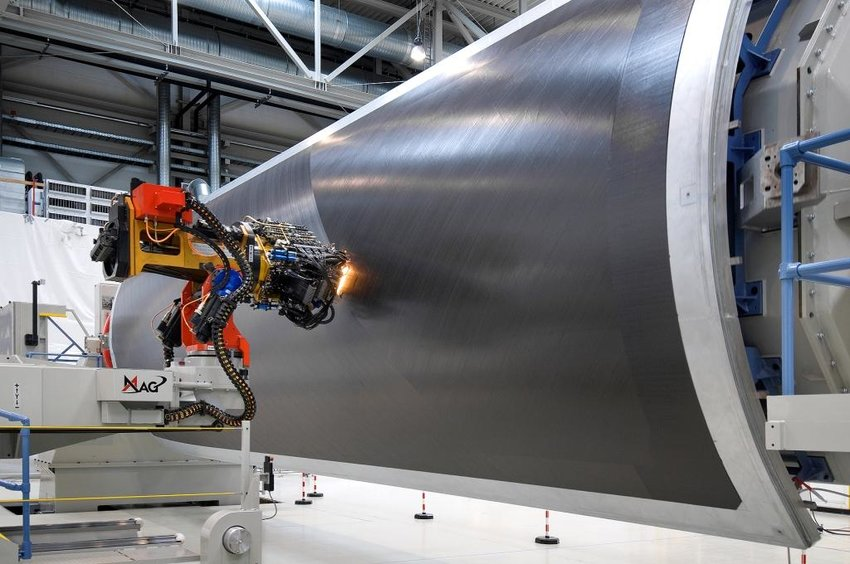
\includegraphics[width=0.75\linewidth]{Fuselaje hecho con AFP.png}
        \caption{Tapa de CFRP (Carbon-fiber-reinforced polymers) para uso aeroespacial}
        \label{fig:enter-label}
    \end{figure}
    \item Automotriz: AFP se puede utilizar para fabricar piezas compuestas para la industria automotriz, como paneles de carrocería, componentes de transmisión y piezas de suspensión.
    \begin{figure}[H]
        \centering
        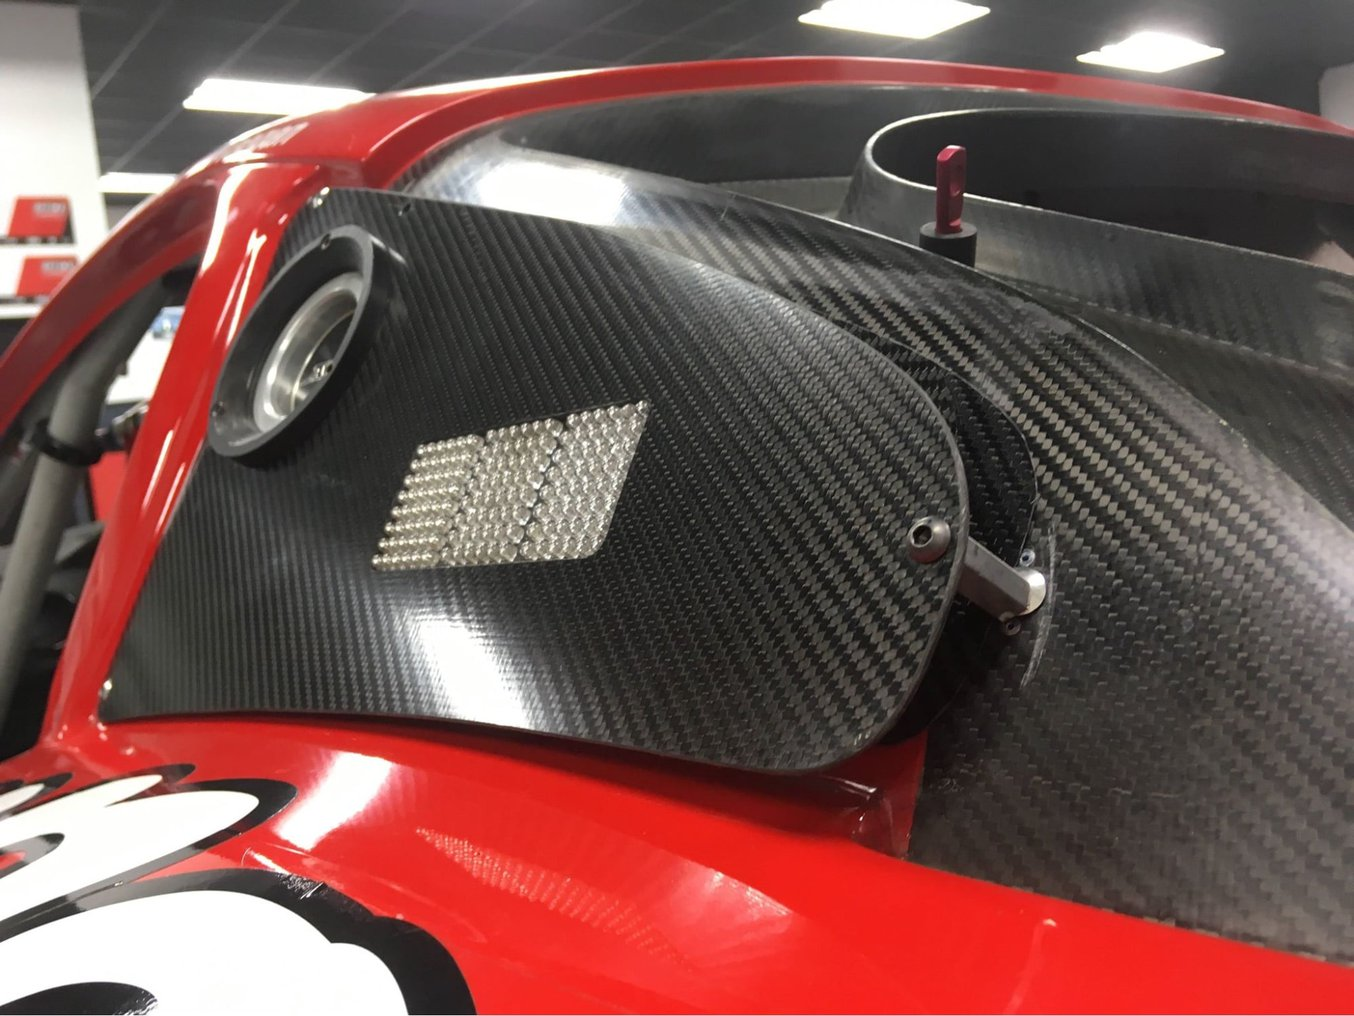
\includegraphics[width=0.5\linewidth]{Pieza de carroceria.png}
        \caption{Pieza de carrocería hecha a base de fibra de carbono}
        \label{fig:enter-label}
    \end{figure}
    \item Construcción: El AFP se puede utilizar para fabricar materiales compuestos para su uso en la construcción, como tableros de puentes, vigas y columnas.
    \item Energía eólica: la AFP se puede utilizar para fabricar palas compuestas de turbinas eólicas, que suelen ser más largas y flexibles que las palas tradicionales.
    \item Artículos deportivos: el AFP se puede utilizar para fabricar materiales compuestos para su uso en artículos deportivos, como palos de golf, raquetas de tenis y esquís.
    \begin{figure}[H]
        \centering
        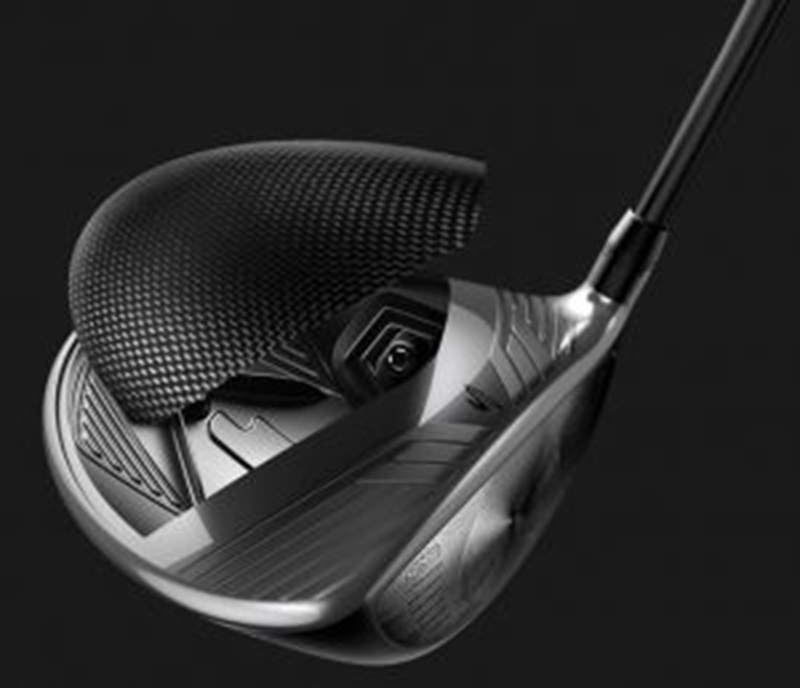
\includegraphics[width=0.5\linewidth]{Articulo deportivo.png}
        \caption{Articulo deportivo fabricado con un material compuesto}
        \label{fig:enter-label}
    \end{figure}
    \item Marina: AFP se puede utilizar para fabricar materiales compuestos para su uso en la industria marina, como cascos de barcos y barcos.
    \item Médico: La AFP se puede utilizar para fabricar materiales compuestos para su uso en dispositivos médicos, como dispositivos implantables y prótesis.
    \item Productos de consumo: la AFP se puede utilizar para fabricar materiales compuestos para su uso en productos de consumo, como productos electrónicos y electrodomésticos.
\end{itemize}
Esta tecnología de laminado es la utilizada para fabricar el cono de cola del avión Airbus A350 XWB.
\begin{figure}[H]
        \centering
        \includegraphics[width=0.70\linewidth]{imagenes/cono de cola A350.png}
        \caption{Fabricación de cono de cola del A350 XWB}
        \label{fig:enter-label}
\end{figure}
    
\section{ATL}

Las aplicaciones típicas en la industria aeroespacial son:
\begin{itemize}
    \item Superficies de control con contornos suaves.
    \begin{figure}[H]
        \centering
        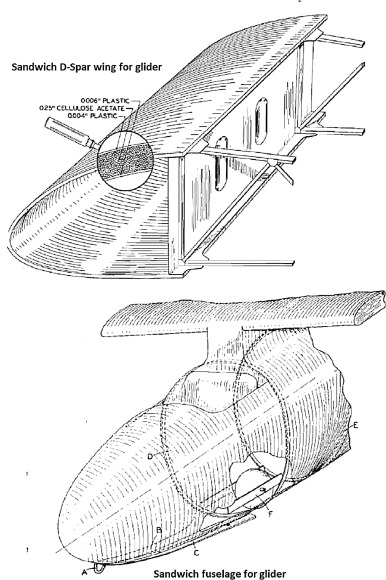
\includegraphics[width=0.35\linewidth]{Superficies de control.png}
        \caption{Componentes estructurales hechos con un material compuesto}
        \label{fig:enter-label}
    \end{figure}
    \item Paneles de fuselaje contorneados.
    \item Secciones de cañón de fuselaje completo.
\begin{figure}[H]
    \centering
    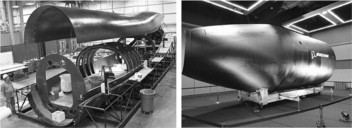
\includegraphics[width=0.8\linewidth]{Secciones de fuselaje.png}
    \caption{Secciones de fuselaje}
    \label{fig:enter-label}
\end{figure}
    \item Carenados contorneados.
    \item Revestimientos de góndola.
    \item Cubiertas/adaptadores de carga útil.
    \item Ejes estructurales (rectos y contorneados).  
    \item Componentes de alas y empenaje.
    \begin{figure}[H]
        \centering
        \includegraphics[width=0.7\linewidth]{imagenes/componente estructural.png}
        \caption{Componente estructural fabricado en ATL}
        \label{fig:enter-label}   
    \end{figure}
\end{itemize}
Si se requiere más contorno, se requeriría una máquina personalizada.

\section{Deposición automática de fibras en la industria aeronáutica}
Debido a las capacidades de este proceso, la industria aeronáutica hace uso de la deposición automática de fibras para la fabricación de múltiples piezas, algunas de las empresas que utilizan este proceso son:
\begin{itemize}
    \item Boeing
    \item Airbus
    \item Spirit Aerosystems
    \item Dassault Aviation
    \item Embraer
    \item GKN Aerospace
\end{itemize}




\textbf{}
\chapter{Capitulo 7. Defectos del proceso}
\label{capitulo 3}
Debido a la complejidad inherente del proceso AFP, la aparición de defectos es inevitable durante todo el laminado. Estos defectos de fabricación pueden tener una influencia negativa significativa en el rendimiento de una estructura, por lo que es vital comprender la creación y el efecto de cada defecto. La mayoría de los defectos son un efecto secundario de la geometría de la herramienta, la dirección de la fibra y las imperfecciones del material. Todos los defectos se pueden dividir en 4 categorías principales: 

\section{Defectos de posicionamiento:}

\begin{itemize}
    \item Un Gap es cuando dos fibras adyacentes no están perfectamente colocadas uno al lado del otro y hay un espacio entre los dos. Una superposición es cuando las dos fibras adyacentes se superponen entre sí. La causa más común de espacios y superposiciones es la dirección durante el lanzamiento, ya que las fibras en un recorrido no encajan perfectamente, especialmente cuando se adopta una estrategia de cobertura paralela. Sin embargo, las lagunas y las superposiciones pueden ocurrir naturalmente fuera de la dirección si se colocan sobre una superficie de herramienta 3D compleja.

\begin{figure}[h]
    \centering
    \includegraphics[width=0.9\linewidth]{eins.png}
    \caption{GAP}
    \label{fig:enter-label}
\end{figure}


\item Defectos de unión: Un Puente es cuando no se adhiere completamente a la superficie cóncava (parte hembra de la herramienta) sobre la que se depositan las fibras, dejando un espacio entre el radio de la superficie cóncava de la herramienta y la fibra. Las principales causas de un Puente son demasiada tensión. En la fibra, lo que la obligará a levantarse, o una adherencia insuficiente a la superficie que se está colocado debido a que el rodillo no proporciona contacto completo con el material del sustrato.

\begin{figure}[H]
    \centering
    \includegraphics[width=0.9\linewidth]{zwei.png}
    \caption{Bridging}
    \label{fig:enter-label}
\end{figure}


\item Defectos de carrete: Cuando el material o el proveedor de corte unen dos cables de extremo a extremo en un carrete mediante superponiendo de 1 a 3 pulgadas entre sí y uniéndolos con tachuelas. Esto da como resultado una porción de el carrete que es más grueso que el resto y suele estar marcado con guiones blancos para su detección. En teoría, las fibras de carbono pueden tener una longitud infinita. Sin embargo, la mayoría de las AFP preimpregnadas son cintas cortadas de un rollo de cinta unidireccional de longitud finita. Estas cintas cortadas son empalmados y enrollados según las especificaciones del cliente.

\begin{figure}[H]
    \centering
    \includegraphics[width=0.9\linewidth]{drei.png}
    \caption{Splice}
    \label{fig:enter-label}
\end{figure}


\item Cuerpos extraños: Foreign object debris (FOD) se produce cuando una pequeña pieza de material compuesto, ya sea carbono “bola de pelusa” o “bola de resina” de fibra que se ha acumulado en las superficies de la cabeza u otros desechos del área de producción cae sobre la pieza durante el laminado. Esto da como resultado un pequeño exceso de volumen de material.sobre la lona si se coloca encima.

\begin{figure}[H]
    \centering
    \includegraphics[width=0.9\linewidth]{vier.png}
    \caption{FOD}
    \label{fig:enter-label}
\end{figure}
\end{itemize}

En la Tabla a continuación se proporciona una lista completa de todos los tipos de defectos y sus categorías.

\begin{figure}[H]
    \centering
    \includegraphics[width=1\linewidth]{funf.png}
    \caption{Defectos}
    \label{fig:enter-label}
\end{figure}


\textbf{}
\chapter{Capitulo 8 Ventajas y Desventajas del proceso}
\label{capitulo 3}


\section{ \textbf{Ventajas}: }
El sistema de deposición automática de fibra tiene la capacidad de variar la velocidad de colocación, la presión, la temperatura y la tensión de las fibras. Todas estas capacidades se complementan con un sistema de programación fuera de línea que beneficiaría el tiempo de producción de la máquina. 
\item 1. Plazos de producción más cortos: las pruebas toman tiempo, pero acortan el plazo total de comercialización y permiten a las partes identificar problemas y abordarlos tempranamente. Encontrar estos problemas más adelante a menudo genera retrasos y cambios costosos e incluso podría exigir rediseños completos de los procesos o equipos de producción.

\item2. Tasas de colocación más rápidas: la velocidad a la que se aplican los materiales compuestos es fundamental. Las rápidas tasas de disposición del material producen una mayor fabricación en todo momento. Las primeras pruebas permiten calibrar los procesos de automatización y formateo de materiales para lograr el proceso de colocación más rápido posible.

\item 3. Menos paradas y cambios: el funcionamiento continuo es tan importante como la velocidad. Al incluir un formateo de precisión como parte del proceso de desarrollo de productos, se pueden minimizar las paradas no planificadas, costosas y que consumen mucho tiempo.

Por ejemplo, el formato y el tamaño del carrete son factores clave en los cambios. El diseño del carrete debe basarse en el tamaño de la pieza, el cronograma de producción y las limitaciones de tiempo para la aplicación específica. Si se necesitan 100 pies de cinta cortada compuesta para fabricar una pieza y se producen seis piezas por día, los carretes deben transportar al menos 600 pies de cinta cortada. De lo contrario, será necesario realizar cambios durante un día de producción, lo que provocará retrasos innecesarios. Además, si el tamaño del carrete es incorrecto para una aplicación, puede surgir un problema de gestión de materiales con carretes remanentes o material costoso desperdiciado debido al tiempo de espera. Parece sencillo, pero incluso este tipo fundamental de planificación afecta al fabricante de materiales y al proveedor de equipos de automatización.
La mala calidad de la cinta también puede provocar tiempos de inactividad. Las cintas que no han sido formateadas correctamente pueden tener bordes irregulares y peludos o tiras que pueden quedar atrapadas y apagar la máquina AFP. Resolver los problemas de tamaño de carrete y calidad de la cinta antes de la producción puede evitar paradas y cambios innecesarios.4. Mayor rendimiento del material: el rendimiento del material generalmente depende de las especificaciones del rollo principal frente al ancho y largo de la cinta formateada, el tamaño y la forma de la pieza fabricada y el tipo de empalmes aceptables en la pieza terminada; también implica compensaciones, como la elección entre cinta compuesta ancha o estrecha.
 Una cinta más ancha permite colocar más material con cada pasada de la máquina, pero también podría haber más desperdicio en los bordes con dientes de sierra. Una cinta más estrecha podría mejorar el rendimiento, pero a costa de más tiempo de producción. Crear anchos de hendidura óptimos y una cantidad de cintas por disposición son vitales para cumplir con los objetivos de rendimiento y costos de producción. La combinación de varios tamaños también puede mejorar el rendimiento sin comprometer el rendimiento.
Resolver estos problemas durante el desarrollo de productos conserva los materiales compuestos, mejora la relación compra-vuelo y reduce los costos de producción. La realización de pruebas tempranas permite a los socios de la cadena de suministro identificar y superar los desafíos y aprovechar las oportunidades para utilizar nuevos materiales, formatos y métodos de fabricación.
\section{ \textbf{Desventajas}: }
En este proceso es imposible controlar de manera precisa el espesor del material compuesto ya que incluso si la pieza sobre la cual se posicionan las fibras tiene una forma cilíndrica perfecta el borde interior del camino curvo no será cubierta de manera perfecta, cuando las imperfecciones de el carrete de fibra como la diferencia del borde se agregan las longitudes y la variación del ancho la distorsión del elemento empeora, en principio, los defectos inducidos por la deformación por flexión en el plano, como la deformación local por pandeo y el cambio de espesor son inevitables, por lo tanto se recomienda que la curvatura del camino del carrete se mantenga al mínimo posible para reducir estos efectos locales. La mayoría de los defectos son provocados por flexión en el plano sobre el cuál se aplican las fibras, el espacio entre las fibras y la superposición de estas provocan que la deformación sea inevitable y aunque la uniformidad del espesor puede ser superior a otros métodos sigue sin ser controlado de manera perfecta.

\textbf{}
\chapter{Capitulo 9 Conclusiones generales del proceso}
\label{capitulo 3}

Desde el inicio industrial de AFP en la década de 1980, ha avanzado continuamente hasta convertirse en una técnica de fabricación líder para grandes estructuras compuestas. Los primeros avances en los ámbitos de la confiabilidad y la productividad de los procesos abren el camino para la adopción de esta técnica en muchas empresas aeroespaciales. Al revisar las complejidades de cada pilar del proceso de las AFP, es evidente que el progreso no se ha estancado. La experiencia que abarca desde el diseño compuesto hasta la inspección proporciona una comprensión profunda del proceso AFP. Este conocimiento ha producido las tecnologías de vanguardia que se presentan aquí. La productividad y la confiabilidad generales siguen aumentando a medida que AFP ingresa al ámbito de la fabricación del futuro.
Con el salto a la Industria 4.0, creemos que el foco de la investigación de AFP debe estar en el aumento del conocimiento experto a través del desarrollo de sistemas expertos, el desarrollo continuo de pequeñas máquinas modulares flexibles y una reducción en el tiempo de producción y el costo de los equipos a través de la Adopción de procesos y materiales OOA. Esto presenta una serie de oportunidades de investigación que culminan en un proceso de AFP de circuito cerrado.

\textbf{}
\include{capitulo_10}
\include{4-capitulo_1}
\include{5-capitulo_2}
\include{6-capitulo_3}
\include{7-conclusiones}
\chapter{Referencias}
\label{Referencias}

\bibitem{bannister2001}
Bannister, M., 2001. Challenges for composites into the next millennium – a reinforcement perspective. Compos. A 31, 901–910.

\bibitem{bardy2012}
Bardy, J., Legrand, X., Crosky, A., 2012. Configuration of a genetic algorithm used to optimise fibre steering in composite laminates. Compos. Struct. 94, 2048–2056.

\bibitem{beasley1993}
Beasley, D., Bull, D.R., Martin, R.R., 1993. An overview of genetic algorithms: Part 1, fundamentals. Univ. Comput. 15 (2), 58–69.

\bibitem{crosky2006}
Crosky, A., Kelly, D., Li, R., Legrand, X., Huong, N., Ujjin, R., 2006. Improvement of bearing strength of laminated composites. Compos. Struct. 76, 260–271.

\bibitem{crosky2012}
Crosky, A., Grant, C., Kelly, D., 2012. Fiber placements. In: Nocolais, N., Borzacchiello, A., Lee, S.M. (Eds.), Wiley Encyclopedia of Composites, second ed. Wiley, Hoboken, NJ, pp. 945–950.

\bibitem{gliesche2003}
Gliesche, K., Hubner, T., Orawetz, H., 2003. Application of the tailored fibre placement (TFP) process for a local reinforcement on an “open-hole” tension plate from carbon/epoxy laminates. Compos. Sci. Technol. 63 (1), 81–88.

\bibitem{goldberg1989}
Goldberg, D.E., 1989. Genetic Algorithms in Search, Optimisation, and Machine Learning. Addison Wesley, Reading, MA.

\bibitem{grant2006}
Grant, C., 2006. Automated processes for composite aircraft structure. Ind. Rob. 33 (2), 117–121.

\bibitem{grant2010}
Grant, C., 2010. Composites automation: there’s a lot of room for growth. In: SME Aerospace \& Defense Manufacturing Yearbook 2010. SME, Dearborn.

\bibitem{grant2012}
Grant, C., 2012. Composites automation: trending smaller and robotic. Compos. World.

\bibitem{honda2011}
Honda, S., Narita, Y., 2011. Vibration design of laminated fibrous composite plates with local anisotropy induced by short fibers and curvilinear fibers. Compos. Struct. 93, 902–910.

\bibitem{kelly2001a}
Kelly, D.W., Willgoss, R., Li, R., Crosky, A., 2001a. Improvement of bearing strength of mechanically fastened composite joints using fibre steering. In: Repecka, L., Saremi, F.F. (Eds.), Proceedings of the 48th International SAMPE Symposium, Long Beach, pp. 2495–2506.

\bibitem{kelly2001b}
Kelly, D.W., Hsu, P., Asadullah, M., 2001b. Load paths and load flow in finite element analysis. Eng. Comput. 18 (1/2), 304–313.

\bibitem{legrand2006}
Legrand, X., Crosky, A., Kelly, D., Crepin, D., 2006. Optimisation of fibre steering in composite laminates using a genetic algorithm. Compos. Struct. 75 (1–4), 524–531.

\bibitem{li2002a}
Li, R., Kelly, D., Crosky, A., 2002a. Strength improvement by fibre steering around a pin loaded hole. Compos. Struct. 57, 377–383.

\bibitem{li2002b}
Li, R., Kelly, D.W., Arima, S., Willgoss, R.A., Crosky, A.G., 2002b. Fiber steering around a cut-out in a shear loaded panel. In: Rasmussen, B.M., Pilato, L.A., Kliger, H.S. (Eds.), Proceedings of the 49th International SAMPE Symposium, Long Beach, pp. 1853–1861.

\bibitem{li2006}
Li, R., Kelly, D., Crosky, A., Schoen, H., Smolich, L., 2006. Joint efficiency of fibre steered composite joint using load path trajectories. J. Compos. Mater. 40 (18), 1645–1658.

\bibitem{peters2011}
Peters, S.T., 2011. Composites Filament Winding. ASM International, Materials Park, OH.

\bibitem{sloan2009}
Sloan, J., 2009. AFP/ATL design to manufacture: bridging the gap. High Perform. Compos.

\bibitem{starr2000}
Starr, T.F., 2000. Pultrusion for Engineers. Woodhead, Cambridge.

\bibitem{tabakov2010}
Tabakov, P.Y., Walker, A., 2010. A technique for stiffness improvement by optimization of fiber steering in composite plates. Appl. Compos. Mater. 17

\bibitem{Miravete}
Miravete, Antonio. 2011. Materiales Compuestos. EDITORIAL REVERTÉ S.A.

\bibitem{Lubin}
Lubin, George. 1982. HANDBOOK OF COMPOSITES. VAN NOSTRAND REINHOLD COMPANY

\bibitem{MIL-HDBK-17-3F}
MIL-HDBK-17-3F. 1997. COMPOSITE MATERIALS HANDBOOK. DISTRIBUTION STATEMENT A.

\bibitem{AMFLSC}
Additive Manufacturing for Lightweight Structural Components. 2023. The Automated Fiber Placement Process: Design Cycle, Benefits, and Applications. 

\bibitem{SAMPE}
Society for the Advancement of Material and Process Engineering. 2011. Automated Tape Laying and Fiber Placement Technologies.

\bibitem{SAMPE}
Mongoose HybridTM - Automatic Fiber Placement Machine by Camozzi Machine Tools | DirectIndustry. (s. f.). https://www.directindustry.com/prod/camozzi-machine-tools/product-26616-2242753.html

\bibitem{SAMPE}
Coriolis Composites: the reference in automated fiber placement. (2022, 13 diciembre). Coriolis. https://www.coriolis-composites.com/

\bibitem{SAMPE}
AddComposites | Plug and Place AFP. (s. f.). Addcomposites. https://www.addcomposites.com/
\textbf{}


\end{document}